% Options for packages loaded elsewhere
\PassOptionsToPackage{unicode}{hyperref}
\PassOptionsToPackage{hyphens}{url}
%
\documentclass[
  english,
  pub,floatsintext]{apa6}
\usepackage{lmodern}
\usepackage{amsmath}
\usepackage{ifxetex,ifluatex}
\ifnum 0\ifxetex 1\fi\ifluatex 1\fi=0 % if pdftex
  \usepackage[T1]{fontenc}
  \usepackage[utf8]{inputenc}
  \usepackage{textcomp} % provide euro and other symbols
  \usepackage{amssymb}
\else % if luatex or xetex
  \usepackage{unicode-math}
  \defaultfontfeatures{Scale=MatchLowercase}
  \defaultfontfeatures[\rmfamily]{Ligatures=TeX,Scale=1}
\fi
% Use upquote if available, for straight quotes in verbatim environments
\IfFileExists{upquote.sty}{\usepackage{upquote}}{}
\IfFileExists{microtype.sty}{% use microtype if available
  \usepackage[]{microtype}
  \UseMicrotypeSet[protrusion]{basicmath} % disable protrusion for tt fonts
}{}
\makeatletter
\@ifundefined{KOMAClassName}{% if non-KOMA class
  \IfFileExists{parskip.sty}{%
    \usepackage{parskip}
  }{% else
    \setlength{\parindent}{0pt}
    \setlength{\parskip}{6pt plus 2pt minus 1pt}}
}{% if KOMA class
  \KOMAoptions{parskip=half}}
\makeatother
\usepackage{xcolor}
\IfFileExists{xurl.sty}{\usepackage{xurl}}{} % add URL line breaks if available
\IfFileExists{bookmark.sty}{\usepackage{bookmark}}{\usepackage{hyperref}}
\hypersetup{
  pdftitle={Effects of human-animal interactions on affect and cognition},
  pdfauthor={Elise R. Thayer1 \& Jeffrey R. Stevens1},
  pdflang={en-EN},
  pdfkeywords={affect, animal-assisted interventions, cognitive performance, executive function, human-animal interaction},
  hidelinks,
  pdfcreator={LaTeX via pandoc}}
\urlstyle{same} % disable monospaced font for URLs
\usepackage{graphicx}
\makeatletter
\def\maxwidth{\ifdim\Gin@nat@width>\linewidth\linewidth\else\Gin@nat@width\fi}
\def\maxheight{\ifdim\Gin@nat@height>\textheight\textheight\else\Gin@nat@height\fi}
\makeatother
% Scale images if necessary, so that they will not overflow the page
% margins by default, and it is still possible to overwrite the defaults
% using explicit options in \includegraphics[width, height, ...]{}
\setkeys{Gin}{width=\maxwidth,height=\maxheight,keepaspectratio}
% Set default figure placement to htbp
\makeatletter
\def\fps@figure{htbp}
\makeatother
\setlength{\emergencystretch}{3em} % prevent overfull lines
\providecommand{\tightlist}{%
  \setlength{\itemsep}{0pt}\setlength{\parskip}{0pt}}
\setcounter{secnumdepth}{-\maxdimen} % remove section numbering
% Make \paragraph and \subparagraph free-standing
\ifx\paragraph\undefined\else
  \let\oldparagraph\paragraph
  \renewcommand{\paragraph}[1]{\oldparagraph{#1}\mbox{}}
\fi
\ifx\subparagraph\undefined\else
  \let\oldsubparagraph\subparagraph
  \renewcommand{\subparagraph}[1]{\oldsubparagraph{#1}\mbox{}}
\fi
% Manuscript styling
\usepackage{upgreek}
\captionsetup{font=singlespacing,justification=justified}

% Table formatting
\usepackage{longtable}
\usepackage{lscape}
% \usepackage[counterclockwise]{rotating}   % Landscape page setup for large tables
\usepackage{multirow}		% Table styling
\usepackage{tabularx}		% Control Column width
\usepackage[flushleft]{threeparttable}	% Allows for three part tables with a specified notes section
\usepackage{threeparttablex}            % Lets threeparttable work with longtable

% Create new environments so endfloat can handle them
% \newenvironment{ltable}
%   {\begin{landscape}\begin{center}\begin{threeparttable}}
%   {\end{threeparttable}\end{center}\end{landscape}}
\newenvironment{lltable}{\begin{landscape}\begin{center}\begin{ThreePartTable}}{\end{ThreePartTable}\end{center}\end{landscape}}

% Enables adjusting longtable caption width to table width
% Solution found at http://golatex.de/longtable-mit-caption-so-breit-wie-die-tabelle-t15767.html
\makeatletter
\newcommand\LastLTentrywidth{1em}
\newlength\longtablewidth
\setlength{\longtablewidth}{1in}
\newcommand{\getlongtablewidth}{\begingroup \ifcsname LT@\roman{LT@tables}\endcsname \global\longtablewidth=0pt \renewcommand{\LT@entry}[2]{\global\advance\longtablewidth by ##2\relax\gdef\LastLTentrywidth{##2}}\@nameuse{LT@\roman{LT@tables}} \fi \endgroup}

% \setlength{\parindent}{0.5in}
% \setlength{\parskip}{0pt plus 0pt minus 0pt}

% \usepackage{etoolbox}
\makeatletter
\patchcmd{\HyOrg@maketitle}
  {\section{\normalfont\normalsize\abstractname}}
  {\section*{\normalfont\normalsize\abstractname}}
  {}{\typeout{Failed to patch abstract.}}
\patchcmd{\HyOrg@maketitle}
  {\section{\protect\normalfont{\@title}}}
  {\section*{\protect\normalfont{\@title}}}
  {}{\typeout{Failed to patch title.}}
\makeatother
\shorttitle{Cognitive effects of HAI}
\keywords{affect, animal-assisted interventions, cognitive performance, executive function, human-animal interaction}
\usepackage{csquotes}
\usepackage[position=top]{subfig}
\usepackage{threeparttable}
\ifxetex
  % Load polyglossia as late as possible: uses bidi with RTL langages (e.g. Hebrew, Arabic)
  \usepackage{polyglossia}
  \setmainlanguage[]{english}
\else
  \usepackage[shorthands=off,main=english]{babel}
\fi
\ifluatex
  \usepackage{selnolig}  % disable illegal ligatures
\fi
\newlength{\cslhangindent}
\setlength{\cslhangindent}{1.5em}
\newlength{\csllabelwidth}
\setlength{\csllabelwidth}{3em}
\newenvironment{CSLReferences}[2] % #1 hanging-ident, #2 entry spacing
 {% don't indent paragraphs
  \setlength{\parindent}{0pt}
  % turn on hanging indent if param 1 is 1
  \ifodd #1 \everypar{\setlength{\hangindent}{\cslhangindent}}\ignorespaces\fi
  % set entry spacing
  \ifnum #2 > 0
  \setlength{\parskip}{#2\baselineskip}
  \fi
 }%
 {}
\usepackage{calc}
\newcommand{\CSLBlock}[1]{#1\hfill\break}
\newcommand{\CSLLeftMargin}[1]{\parbox[t]{\csllabelwidth}{#1}}
\newcommand{\CSLRightInline}[1]{\parbox[t]{\linewidth - \csllabelwidth}{#1}\break}
\newcommand{\CSLIndent}[1]{\hspace{\cslhangindent}#1}

\title{Effects of human-animal interactions on affect and cognition}
\author{Elise R. Thayer\textsuperscript{1} \& Jeffrey R. Stevens\textsuperscript{1}}
\date{}


\authornote{

Department of Psychology, Center for Brain, Biology \& Behavior, University of Nebraska, Lincoln, Lincoln, NE, USA 68588

The authors made the following contributions. Elise R. Thayer: Conceptualization, Data Curation, Formal Analysis, Investigation, Methodology, Project Administration, Software, Supervision, Visualization, Writing - Original Draft Preparation, Writing - Review \& Editing; Jeffrey R. Stevens: Conceptualization, Data Curation, Methodology, Resources, Software, Supervision, Validation, Writing - Review \& Editing.

Correspondence concerning this article should be addressed to Jeffrey R. Stevens, B83 East Stadium, University of Nebraska-Lincoln, Lincoln, NE 68588. E-mail: \href{mailto:jeffrey.r.stevens@gmail.com}{\nolinkurl{jeffrey.r.stevens@gmail.com}}

}

\affiliation{\vspace{0.5cm}\textsuperscript{1} University of Nebraska-Lincoln}

\abstract{
Human-animal interaction has clear positive effects on people's affect and stress. But less is known about how animal interactions influence cognition. We draw parallels between animal interactions and exposure to natural environments, a research area that shows clear improvements in cognitive performance. The aim of this study is to investigate whether interacting with animals similarly enhances cognitive performance, specifically executive functioning. To test this, we conducted two experiments in which we had participants self-report their affect and complete a series of cognitive tasks (long-term memory, attentional control, and working memory) before and after either a brief interaction with a dog or a control activity. We found that interacting with a dog improved positive affect and decreased negative affect (in one of the two experiments), stress, and anxiety compared to the control condition. However, we did not find effects of animal interaction on long-term memory, attentional control, or working memory. Thus, we replicated existing findings providing evidence that interacting with animals can improve affect, but we did not find similar improvements in cognitive performance. These results suggest that either our interaction was not of sufficient dose or timed appropriately to elicit effects on cognition or the mechanisms underlying effects of human-animal interaction on cognition differ from effects generated by other cognition-enhancing interventions such as exposure to nature. Future research should continue to increase knowledge of the connection between nature exposure and human-animal interaction studies to build our understanding of cognition in response to animal interactions.
}



\begin{document}
\maketitle

\hypertarget{introduction}{%
\section{Introduction}\label{introduction}}

Imagine that you have an hour-long lunch break to take your dog for a walk. Would you rather take Fido down a city street or down a tree-shrouded trail? If you chose the leafy trail, it's not by chance---there is a mountain of evidence to suggest that exposure to natural landscapes is psychologically restorative. Specifically, nature exposure has been shown to increase positive mood (e.g., Mayer et al., 2008), decrease feelings of anxiety (e.g., Bratman et al., 2015), decrease psychological and physiological responses to stress (e.g., Gidlow et al., 2016), and improve cognitive functioning (e.g., Berman et al., 2008; Bratman et al., 2012). The aim of this study is to investigate whether interacting with animals has a similar effect on well-being and cognition as exposure to nature.

At the core of the scientific endeavor to quantify the influence of natural landscapes on human health and well-being is the \emph{biophilia} hypothesis, which postulates that humans have an innate tendency toward and affinity for life and life-like processes (Wilson, 2009). Two relevant theories based on the biophilia hypothesis have been proposed to account for effects of exposure to nature on well-being and cognition. First, \emph{Stress Reduction Theory} proposes that aesthetic features of nature reduce autonomic responses to stress captured by decreases in physiological and experiential indicators of stress (Ulrich, 1981). Second, \emph{Attention Restoration Theory} postulates that experiences in nature restore cognition by replenishing attentional capacities (Kaplan \& Kaplan, 1989; Kaplan, 1995). In this view, an individual requires a finite and exhaustible mental resource to maintain focus on a particular task without distraction (i.e., to maintain directed attention). In turn, this resource can be restored while engaging in tasks or activities that do not require marked cognitive demand, such as interacting with nature.

Though directed attention itself is not clearly defined or quantifiable, it is a key component of executive functions (i.e., those related to complex, goal-directed behaviors) and can be tested with well-established paradigms (Miyake et al., 2000). For example, researchers have investigated the effects of experiences in nature on executive functions such as \emph{attentional control} (i.e., the ability to simultaneously attend to relevant information and ignore distracting information) and \emph{working memory} (i.e., the ability to mentally hold and manipulate information in the short-term). The improvement in cognitive performance often observed following nature exposure thereby provides evidence for the restorative effects of nature (for a review, see Stevenson et al., 2018). Though some researchers posit that decreases in stress facilitate attention restoration, evidence indicates that autonomic and cognitive effects of exposure to natural landscapes are distinguishable (Li \& Sullivan, 2016). As such, the quantification of nature's influence on cognition is concentrated in research working through the Attention Restoration framework.

The study of human-animal interactions---the mutual and dynamic exchanges between humans and non-human animals (Griffin et al., 2019)---also rests on the same foundational principle of biophilia, though it is minimally integrated with the nature exposure literature (but see Franco et al., 2017). Yet human-animal interactions (HAIs) elicit strikingly similar effects on human health and well-being as nature exposure. Human-animal interactions encompass the interactions between owners and pets, handlers and trained service dogs, and individuals and unfamiliar dogs (Thayer \& Stevens, 2019b). This is of particular public interest in light of the rapidly increasing presence of dogs in hospitals, schools, and therapeutic contexts (Barker \& Wolen, 2008; Friedmann \& Son, 2009; Hosey \& Melfi, 2014). Here, we focus on animal-assisted interventions or facilitated interactions between an unfamiliar animal and a person to improve individual health or well-being (Thayer \& Stevens, 2019a). These interactions between individuals and unfamiliar dogs can evoke positive mood (Beetz et al., 2012; Crossman et al., 2020) and mitigate behavioral and physiological responses to stress (Odendaal \& Meintjes, 2003; Lass-Hennemann et al., 2014; Barker et al., 2016; Fiocco \& Hunse, 2017; Ein et al., 2018). However, these effects are not always present. For example, Johnson et al. (2008) found no effect of canine-assisted activities on mood, and Barker et al. (2003) found no effect on anxiety.

Akin to the understanding that human preferences for natural views are evolved, HAI practitioners believe the stress- and anxiety-reducing effects of animal interactions to be largely a function of humans' evolutionary need to attend to environmental cues for survival, animals being key indicators of environmental safety (Serpell, 1996; Kruger \& Serpell, 2010). In turn, it is assumed that there are subconscious feelings of safety elicited by these benign interactions that induce a calming effect that reduces stress (Beetz, 2017). Since animal interactions and natural experiences elicit similar stress-reducing effects, do human-animal interactions possess the same cognitive restorative potential as experiences in nature?

There is a gap in the human-animal interaction literature with regard to the place of HAIs in relation to cognitive performance. HAIs and cognitive performance in adults are disproportionately understudied compared to the presence of HAIs in educational contexts (Gee et al., 2017). There have been few direct tests of HAIs and cognitive performance in adults (Gee et al., 2014, 2015; Trammell, 2019) or children (Gee et al., 2010, 2012; Hediger \& Turner, 2014). Most of these studies approached cognition from a bio-psycho-social model of stress reduction, analogous to Stress Reduction Theory. Trammell (2019) replicated effects of human-dog interactions on self-reported affect but found no differences between control and HAI groups' performance in a long-term memory paradigm. Long-term memory, however, is not a part of the executive function system, so it is perhaps unsurprising that it is not influenced by HAI. Working memory and attentional control, on the other hand, are components of executive function (McCabe et al., 2010). Yet interacting with a dog does not seem to influence working memory in adults (Gee et al., 2014, 2015) or attentional control in children (Hediger \& Turner, 2014). With so few studies, we need to quantify the influence of HAIs on cognition.

Our aim in the present study was to examine the influence of human-animal interactions on affect and cognitive performance in adults using established methods from the adjacent exposure to nature literature. In Experiment 1, we sought to replicate positive affective effects of HAIs observed in previous research (Beetz et al., 2012; Thelwell, 2019; Crossman et al., 2020) and test whether HAI induces restorative effects on cognition using tasks implemented in the experience in nature literature (e.g., Berman et al., 2008). We selected tests of cognitive performance used in the nature exposure literature to capture the attentional control and working memory components of directed attention. We also included a long-term memory task to assess cognitive performance outside of directed attention to investigate if HAI effects might influence cognition generally or executive functioning specifically. We hypothesized that HAI would evoke greater improvements in mood and directed attention but not long-term memory compared to a control condition. We tested these hypotheses using a between-groups pre-post intervention design where we administered affective and cognitive tasks both before and after either a three-minute human-animal interaction or control activity. Further, due to potential moderating effects of affect and pet attitudes on interaction efficacy (Barker et al., 2010), we conducted exploratory moderation analyses of positive and negative affect change and pet attitudes on the effect of animal interaction on cognition. In Experiment 2, we sought to replicate our findings and also replicate self-reported stress- and anxiety-reducing effects of HAI observed in previous research (e.g., Grajfoner et al., 2017) to better characterize the influence of animal interaction on cognition.

\hypertarget{experiment-1}{%
\section{Experiment 1}\label{experiment-1}}

\hypertarget{methods}{%
\subsection{Methods}\label{methods}}

\hypertarget{participants}{%
\subsubsection{Participants}\label{participants}}

We recruited participants who did not have a physical or emotional aversion to dogs (i.e., allergy, fear) from the University of Nebraska-Lincoln (UNL) Department of Psychology subject pool between Sep to Nov 2018. When recruiting participants, we did not include any information about dogs in the study description to avoid introducing self-selection bias into our sample. We also did not include references to dogs in the consent procedure to avoid building expectations about interacting with dogs. We collected data from 73 undergraduate students of whom 60 (82.2\%) identified as female, 13 (17.8\%) identified as male, and 0 (0.0\%) identified as neither female nor male (race/ethnicity and parental income information available in Table S1). Participants were on average 19.2 (\emph{SD} = 1.4) years of age. There were 39 individuals (53.40\%) who currently lived with at least one pet in their primary residence and 62 (84.90\%) who lived with at least one pet as a child. All participants received one hour of research credit in exchange for their participation.

\hypertarget{measures}{%
\subsubsection{Measures}\label{measures}}

Unless otherwise indicated, all stimuli were presented and all responses were collected with Psychopy version 1.90.2 (Peirce et al., 2019) on a computer with a 16 inch monitor in a private room with only the participant and experimenter present.

\textbf{\emph{Affect.}}
We assessed participants' affect with the Positive and Negative Affect Schedule {[}PANAS; Watson et al. (1988){]}. Participants viewed 10 positive and 10 negative adjectives (e.g., ``excited,'' ``disinterested'') and rated each from one (\emph{very slightly or not at all}) to five (\emph{extremely}) as they pertained to how they felt. Higher values for positive adjectives represent more positive affect, and higher values for negative adjectives represent more negative affect. We calculated Revelle's omega total (\(\omega\)) as our measure of internal consistency reliability of scales (Revelle \& Zinbarg, 2008; McNeish, 2018): \(\omega\)\textsubscript{positive} = 0.90, \(\omega\)\textsubscript{negative} = 0.92).

\textbf{\emph{Cognitive tasks.}}
We administered four separate cognitive tasks: Deese-Roedinger-McDermott (long-term memory), Necker cube pattern control (attentional control), backwards digit span (working memory), and n-back (working memory).

\emph{Deese-Roedinger-McDermott.}
We used the Deese-Roedinger-McDermott long-term memory (DRM) paradigm to examine participants' capacity for long-term memory retention (Roediger \& McDermott, 1995; McEvoy et al., 1999). While this task is primarily used for studying false memory, it can be used as a general memory distortion task as well (MacDuffie et al., 2012; Cadavid \& Beato, 2016). During the presentation phase of this task, participants passively viewed two sets of ten words associated with a not-presented critical word (e.g., child) presented one at a time. In the recall phase at the end of the experiment, participants were told that they would view some of the words they were instructed to remember at the beginning of the experiment. They viewed 6 of the 20 previously presented words, the two critical words, and four unrelated words in random order and responded via key press whether they recalled seeing the words previously in the experiment (Table S2). We analyzed mean accuracy as the proportion of items correctly recognized, with 1 representing perfect recognition and 0 representing complete lack of recognition. We also calculated \(d'\) as \(z(P(recall|presented\ word))\) \(-\) \(z(P(recall|not\ presented\ word))\) (Tajika, 2001), but the outcomes are identical to accuracy, so we only report the accuracy results.

\emph{Necker Cube Pattern Control.}
We used the Necker Cube Pattern Control Test to measure participants' attentional control (Orbach et al., 1963; Cimprich, 1993; Sahlin et al., 2016). The Necker cube is an optical illusion that consists of a cube outline that lacks visual cues to indicate its orientation (Figure S1a); with continued viewing, the viewer observes shifts in perspective between back-in-focus and front-in-focus. In this task, participants were prompted to observe the cube and record perceived perspective shifts for 30 s. After this initial trial, they were prompted to observe the cube in a second trial while purposefully holding each focus for as long as possible and minimizing shifts. We calculated the difference in the number of shifts reported between the first and second trials as a measure of participants' attentional control. Positive values represent more shifts in the first trial, which can be interpreted as exerting more attentional control in the second trial.

\emph{Backwards digit span.}
We presented participants with a backwards digit span task to measure their working memory capacity (Berman et al., 2008). In this task, participants viewed sequences of numbers presented individually for one second each, then wrote the sequence down on a sheet of paper in the reverse order from which it was presented (Figure S1b). Following a practice sequence of numbers, participants responded to a total of 14 unique sequences that increased in span (number of digits), starting with three digits and ending with nine digits. We pseudo-randomly generated each sequence such that no digit was repeated within a given sequence. If the participant correctly recorded an entire sequence in reverse order, that response was coded as correct. We measured performance by identifying participants' digit span index, or the greatest span they reversed correctly before failing two consecutive sequences of the same length (Schutte et al., 2017). Spans ranged from 3-9 digits, so higher values represent greater spans, which can be interpreted as better working memory.

\emph{N-back.}
We administered an n-back task as an additional measure of working memory capacity (Cohen et al., 1994; Rich, 2007). In this task, participants observed a stream of phonologically distinct letters {[}B, F, K, H, M, Q, R, X; Kane et al. (2007){]} and responded when the current stimulus was presented \emph{n} (two) trials prior (Figure S1c). Each letter was presented for 0.5 seconds and followed by a 2.5 second inter-stimulus interval (fixation cross). Participants completed a brief practice before viewing a total of 96 letters, of which 16-19 were targets (i.e., matching the stimulus from two trials prior). We assessed participants' working memory performance on the n-back task by calculating \(d'\) as \(z(P(hit|target))\) \(-\) \(z(P(hit|not\ target))\) to capture both correct recognition and false alarm rates (Tajika, 2001). A value of 0 indicates that a participant was not able to discriminate between previously presented and not presented words and larger values indicate greater propensities to discriminate between presented and not-presented words (Haatveit et al., 2010). Higher values can be interpreted as better working memory.

\textbf{\emph{Animal-related measures.}}
In addition to standard demographic metrics (e.g., age and sex), at the end of the experiment, we asked participants whether they owned pets as a child and whether they currently owned pets. We also assessed participants' attitudes towards pets with the Pet Attitude Scale {[}PAS; Templer et al. (1981); Templer et al. (2004){]}. Participants rated the extent to which they agreed with 18 statements (e.g., ``House pets add happiness to my life, or would if I had one'') on a scale from one (strongly disagree) to seven (strongly agree) (\(\omega\) = 0.93). Higher values represent more positive attitudes toward pets.

For those assigned to the HAI condition, we administered an additional questionnaire used by Gee et al. (2015) to assess participants' evaluation of the quality of the dog interaction. Participants rated on a scale from one (strongly disagree) to four (strongly agree) the extent to which they agreed with 11 statements (e.g., ``I felt more relaxed when the dog was present'') pertaining to their comfort, discomfort, ambivalence, and desire to interact with the dog (\(\omega\) = 0.88). Higher values represent more positive experiences with the interaction.

\textbf{\emph{Cardiovascular activity.}}
Participants wore an Empatica E4 wristband on their left wrist for the duration of the experiment to provide a continuous measure of cardiovascular activity, specifically heart rate variability (McCarthy et al., 2016; Empatica, 2018). The E4 wristband uses a photoplethysmogram (PPG) sensor located on the backside of the device face seated atop the wearer's wrist that samples heart beats at 64 Hertz. We do not provide analyses of cardiovascular data because the device did not sample at a sufficient frequency to detect fine changes in heart rate variability (Shaffer \& Ginsberg, 2017).

\hypertarget{procedures}{%
\subsubsection{Procedures}\label{procedures}}

Participants were pseudo-randomly assigned to either an animal interaction (\emph{human-animal interaction} or \emph{HAI}) or control condition before arrival. After participants arrived to the experimental session, they completed informed consent and sat calmly for three minutes to attain a resting state. Then, the researcher instructed the participant to begin the experiment on the computer at their desk. The researcher remained seated in the room throughout the duration of the experiment. The experiment was partitioned into three components, pre-condition, condition, and post-condition, which correspond to the time before, during, and after the animal interaction or control activity, respectively. Participants took about 45 minutes to complete the study.

\textbf{\emph{Pre-condition.}}
Participants experienced the task set in the following order: PANAS, DRM (presentation phase), Necker cube, digit span, and n-back. We administered the affect task first to capture affect upon arrival, the DRM second to allow time to elapse between presentation and recall phases, then followed these with the remaining cognitive tasks in a fixed order for the sake of simplicity.

\textbf{\emph{Condition.}}
Participants experienced three minutes of either the HAI or control condition. We based this timing on changes observed in cortisol, oxytocin, and heart rate after a three-minute dog interaction in Handlin et al. (2011). Participants were not informed which of the three-minute conditions they were assigned to experience until the pre-condition phase was completed.

\emph{HAI.} We employed JRS's pet dog for every animal-interaction session. The dog used for the HAI condition was a 65-pound, neutered, male Catahoula leopard mix that was Canine Good Citizen certified. Prior to this study, he had completed approximately 35 similar sessions in a previous study. When not interacting with participants, the dog was housed in JRS's office or adjacent experiment room that were both equipped with a large kennel and access to water. The dog participated in 1-5 sessions spread throughout the day with at least 40 minutes between sessions. JRS was not involved in the actual behavioral testing or human-animal interaction to minimize potential bias. Researchers monitored the dog for signs of stress (e.g., excessive panting or licking, avoidance of interacting with participants, barking, aggression, fatigue) and stopped the interaction if he showed signs of stress. Signs of stress where never observed during a session, but if they occurred prior to a session, we reassigned the subsequent participant from the HAI to the control condition.

Before introducing participants to the dog, the researcher asked participants if they had a physical or emotional aversion to dogs; no participants reported any dog aversions. The researcher then brought in the dog, inviting the participant to pet and verbally interact with the dog calmly: ``Feel free to pet {[}dog name{]} and talk with him all you want. Please try not to rile him up. Other than that, we'll get back to it in a few minutes.'' Participants were not required to interact with the dog for the whole three minutes.

Participants remained seated for the duration of the interaction. If participants asked questions of or made conversation with the researcher, the researcher briefly informed participants that they would be able to discuss more at the end of the experiment. The dog remained in the experiment room within visual contact after the animal interaction period to rest next to the researcher.

After the experiment ended, researchers debriefed participants who experienced the HAI condition. The researcher explained that participants were not made aware of the dog in recruitment or consent materials to avoid biasing the sample and the results. Researchers requested that participants not discuss the presence of the dog in the experiment with other individuals to help maintain an unbiased sample. Then, researchers invited participants to ask any questions about the nature of the study.

\emph{Control.}
Researchers provided participants with a sheet of paper with a full page of Latin text printed on it and instructed them to circle every `e' and `f' for ``the next few minutes.'' Researchers emphasized that the task would not be graded and incorrect answers would incur no penalty. The researcher collected the sheet after the three minutes passed; no data were extracted from the activity.

\textbf{\emph{Post-condition.}}
Participants completed the tasks again in the following order: PANAS, Necker cube, digit span, n-back, and DRM (recall phase). They then completed the Pet Attitude Scale, and those assigned to the HAI condition also completed the animal experience questionnaire. All participants answered standard and animal-related demographic questions (e.g., age, number of pets owned) to conclude the experiment.

\textbf{\emph{Ethics.}}
All procedures were conducted in an ethical and responsible manner, in full compliance with all relevant codes of experimentation and legislation and were approved by the UNL Internal Review Board (protocol \# 19552) and Institutional Animal Care and Use Committee (protocol \# 1599). All participants gave written consent to participate, and they acknowledged that de-identified data could be published publicly.

\hypertarget{analysis}{%
\subsubsection{Analysis}\label{analysis}}

We analyzed data from 73 participants, with 36 participants experiencing the animal-interaction condition and 37 experiencing the control condition. The sample size was based on previous studies showing effects of HAI on stress responses (Lass-Hennemann et al., 2014; Crossman et al., 2015) with some additional participants added to boost power.

\textbf{\emph{Participant characteristics.}}
We compared pre-condition scores for affective measures, cognitive tasks, and animal-related measures (PAS, pet history) between animal interaction and control groups using independent samples t-tests (or Wilcoxon rank sum test in the case of test violations) to ensure that any experimental differences could not be attributed to participant characteristics. There were no significant between-group differences in any measure (Table \ref{tab:expt1scores}).

\textbf{\emph{Data analysis.}}
We used R {[}Version 4.0.4; R Core Team (2020){]} and the R-packages \emph{BayesFactor} {[}Version 0.9.12.4.2; Morey and Rouder (2018){]}, \emph{ggbeeswarm} {[}Version 0.6.0; Clarke and Sherrill-Mix (2017){]}, \emph{ggcorrplot} {[}Version 0.1.3; Kassambara (2019){]}, \emph{here} {[}Version 1.0.1; Müller (2017){]}, \emph{Hmisc} {[}Version 4.4.2; Harrell Jr et al. (2020){]}, \emph{papaja} {[}Version 0.1.0.9997; Aust and Barth (2020){]}, \emph{patchwork} {[}Version 1.1.1; Pedersen (2020){]}, \emph{psych} {[}Version 2.0.12; Revelle (2019){]}, \emph{rcompanion} {[}Version 2.3.26; Mangiafico (2020){]}, and \emph{tidyverse} {[}Version 1.3.0; Wickham et al. (2019){]} for all our analyses. We prepared the manuscript using \emph{rmarkdown} {[}Version 2.6; Xie et al. (2018){]} and \emph{papaja} {[}Version 0.1.0.9997; Aust and Barth (2020){]}. Data, analysis scripts, supplementary methods, tables, and figures, and the reproducible research materials are available in Supplementary Materials at the Open Science Framework (\url{https://osf.io/v7wxt/}).

In addition to frequentist analyses, we calculated and drew inferences based on Bayes factors, that is, the strength of evidence for the alternative over the null hypothesis. For example, \(BF\) = 15 suggests that there is 15 times more evidence for the alternative than the null hypothesis. Bayes factors between 3-10 provide moderate evidence for the alternative hypothesis, those between 10-30 provide strong evidence, those between 30-100 provide very strong evidence, and those above 100 provide extreme evidence; reciprocal values (1/3, 1/10, 1/30, 1/100) provide comparable evidence for the null hypothesis (Wagenmakers et al., 2018). We used the \emph{BayesFactor} package to calculate most Bayes factors (using default priors and settings), except for the Wilcoxon rank sum tests, which we calculated from code provided by van Doorn et al. (2020).

\emph{Condition effects.}
To assess potential condition differences pre-condition, we conducted independent samples t-tests or Wilcoxon rank sum tests in the case of test violations. For condition effects, we used analysis of covariance to examine the effects of condition on post-scores controlling for pre-scores. We report predicted marginal means and 95\% confidence intervals and calculated effect sizes with generalized eta squared (\({\eta}^2_G\)). We used both visual and test-based methods to check analysis of covariance test assumptions: linearity between covariate and outcome variable, homogeneity of regression slopes, normally distributed residuals on outcome variable, and homogeneity of variance (Johnson, 2016). Since we recorded responses only at post-condition for the long-term memory task, we compared between-groups differences with a Wilcoxon rank sum test, as it violated assumptions of an independent samples t-test. For these, we calculated effect sizes with \(r\), the z-score of the test statistic divided by the total number of observations.

The analyses of covariance for negative affect and Necker cube significantly violated model assumptions, so we log-transformed negative affect pre- and post-scores and removed outliers (standard deviation \(\times\) 3; 2 observations) from Necker post-scores to conform to model assumptions. We excluded one observation from DRM (participant expressed comprehension issues after task), three from Necker cube (participants expressed comprehension issues after task), and three from digit span (participants did not request response sheet) when running respective analyses, inserting missing data for these subjects.

\emph{Moderation analyses.}
We conducted follow-up exploratory analyses to identify potential moderators of the relationship between animal interaction and cognitive performance. Because we have three cognitive measures and several potential moderators, combining all of these would result in a large number of statistical tests. To reduce the number of statistical tests run, we aggregated all of the cognition scores into a single composite measure, as used in the nature exposure literature. Following Van Hedger et al. (2019), we constructed the cognitive composite measure by averaging the z-scores for the Necker cube, digit span, and n-back post - pre difference scores. We tested whether positive and negative affect change (i.e., post - pre difference scores; PANAS) and pet attitude (PAS) explained the relationship between experimental condition and composite cognitive performance change. For each moderation analysis, we used multiple linear regression with predictors \emph{condition}, \emph{moderator}, and \emph{condition}\(\times\)\emph{moderator} and outcome \emph{post - pre cognitive composite}. We report model fit results alone, as no moderation model accounted for more than a negligible amount of the variance in the data.

\emph{Animal experience correlations.}
We also conducted follow-up exploratory analyses to identify correlations between the animal-related measures, affect, and cognitive performance composite.

\begin{table*}

\caption{\label{tab:expt1scores}Experiment 1 scores}
\centering
\resizebox{\linewidth}{!}{
\begin{threeparttable}
\begin{tabular}[t]{lrrrrrrrrrr}
\toprule
\multicolumn{1}{c}{} & \multicolumn{5}{c}{Pre-condition} & \multicolumn{5}{c}{Post-condition} \\
\cmidrule(l{3pt}r{3pt}){2-6} \cmidrule(l{3pt}r{3pt}){7-11}
Measure & $n$ & Control $M$ & HAI $M$ & $p$ & $BF$ & $n$ & Control $M$ & HAI $M$ & $p$ & $BF$\\
\midrule
\addlinespace[0.3em]
\multicolumn{11}{l}{\textbf{Pet measures}}\\
\hspace{1em}Pets now (\%) & 73 & 72.97 & 33.33 & -- & -- & -- & -- & -- & -- & --\\
\hspace{1em}Pets as a child (\%) & 73 & 91.89 & 77.78 & -- & -- & -- & -- & -- & -- & --\\
\hspace{1em}Pet attitude (PAS) & 73 & 5.74 & 5.63 & 0.84 & 0.18 & -- & -- & -- & -- & --\\
\addlinespace[0.3em]
\multicolumn{11}{l}{\textbf{Affective measures}}\\
\hspace{1em}Positive affect (PANAS) & 73 & 3.04 & 2.83 & 0.24 & 0.44 & 73 & 2.74 & 3.25 & < 0.001 & > 100\\
\hspace{1em}Negative affect (PANAS) & 73 & 1.45 & 1.51 & 0.79 & 0.17 & 73 & 0.29 & 0.21 & 0.04 & 1.50\\
\addlinespace[0.3em]
\multicolumn{11}{l}{\textbf{Cognitive tasks}}\\
\hspace{1em}Accuracy (DRM) & -- & -- & -- & -- & -- & 72 & 0.76 & 0.77 & 0.70 & 0.19\\
\hspace{1em}Average shifts (NCPC) & 70 & -0.76 & -1.12 & 0.63 & 0.27 & 70 & -2.41 & -1.66 & 0.39 & 0.34\\
\hspace{1em}Index (Digit span) & 70 & 6.69 & 6.12 & 0.25 & 0.31 & 70 & 7.11 & 7.30 & 0.58 & 0.28\\
\hspace{1em}$d'$ (N-back) & 73 & 0.08 & -0.08 & 0.74 & 0.20 & 73 & 0.04 & -0.04 & 0.73 & 0.26\\
\bottomrule
\end{tabular}
\begin{tablenotes}
\item \textit{Note: } 
\item Post-condition scores control for pre-condition scores.
\end{tablenotes}
\end{threeparttable}}
\end{table*}

\hypertarget{results}{%
\subsection{Results}\label{results}}

\hypertarget{affect}{%
\subsubsection{Affect}\label{affect}}

To test the effect of animal interaction on affect, we compared positive and negative PANAS scores following the control and HAI condition. Figure \ref{fig:panasa} shows the effect of condition on positive and negative affect (Table \ref{tab:expt1scores}; Figure S2). Analyses of covariance indicate very strong evidence that positive affect is greater post-condition for those who experienced HAI than those who did not, controlling for pre-interaction scores (\(F(1, 70) = 30.21\), \(\mathit{MSE} = 0.15\), \(p < .001\), \(\hat{\eta}^2_G = .301\), \(BF\) \textgreater{} 100). For negative affect, on the other hand, there is not sufficient evidence to determine whether the log post-condition scores differed between control and HAI groups (\(F(1, 70) = 4.32\), \(\mathit{MSE} = 0.03\), \(p = .041\), \(\hat{\eta}^2_G = .058\), \(BF\) = 1.50).



\begin{figure*}
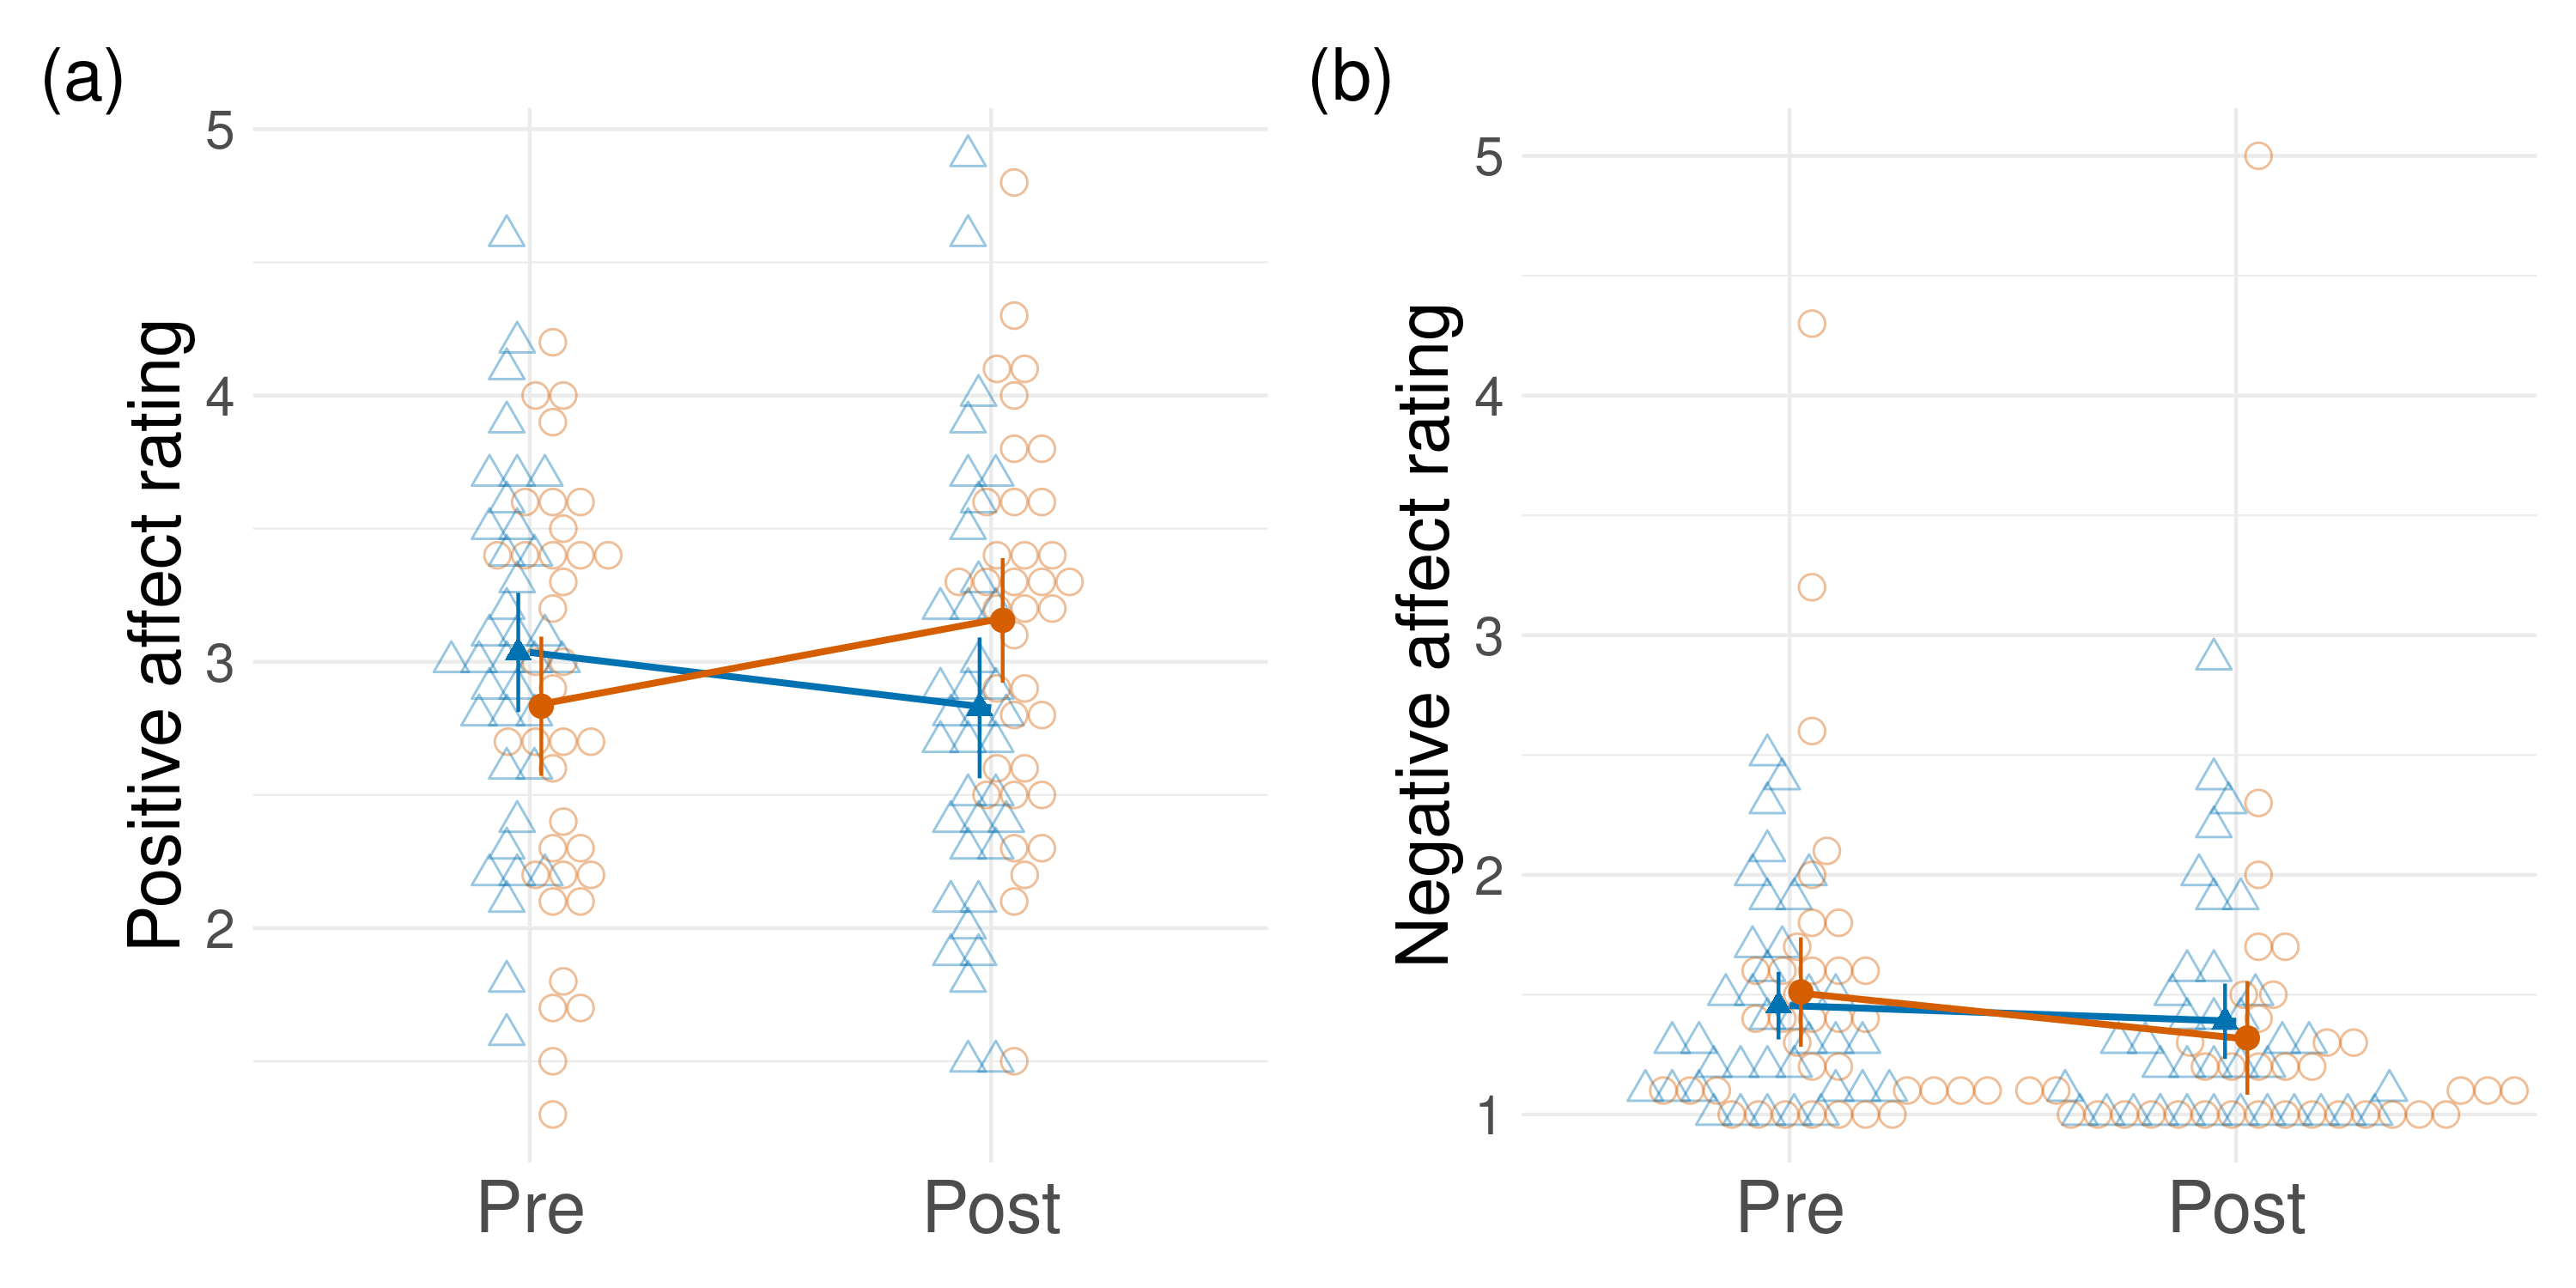
\includegraphics[width=0.9\linewidth]{/mnt/data/jstevens/OneDrive/active_sync/projects/haicognition2021/figures/affect_prepost_1} \caption{Affect scores pre- and post-condition for control and HAI (human-animal interaction) groups in Experiment 1. Scores show (a) positive PANAS ratings and (b) negative PANAS ratings. Open triangles (blue) represent individual control participant scores, open circles (orange) represent individual HAI participant scores, closed triangles and circles represent condition group means (with lines connecting condition means), error bars represent 95\% confidence intervals.}\label{fig:panasa}
\end{figure*}

\hypertarget{cognitive-tasks}{%
\subsubsection{Cognitive tasks}\label{cognitive-tasks}}

To test the effect of animal interaction on cognition, we compared scores on four cognitive tasks following control and HAI conditions. There is evidence to suggest that animal interaction and control groups did not differ on any cognitive task post-condition (Table \ref{tab:expt1scores}; Figures \ref{fig:cognitivea} and S3). Specifically, there is moderate evidence that there is no difference between control and HAI groups for accuracy in the long-term memory task post-condition scores (\(W = 681.00\), \(p = .696\), \(r\) = 0.05, \(BF\) = 0.19). Similarly, the analyses of covariance provide evidence of no difference between groups---controlling for pre-condition scores---for the number of switches in the Necker cube attentional control task (\(F(1, 67) = 0.76\), \(\mathit{MSE} = 12.85\), \(p = .385\), \(\hat{\eta}^2_G = .011\), \(BF\) = 0.34), the backwards digit span index for working memory (\(F(1, 67) = 0.31\), \(\mathit{MSE} = 1.98\), \(p = .578\), \(\hat{\eta}^2_G = .005\), \(BF\) = 0.28), and the n-back \(d'\) for working memory (\(F(1, 70) = 0.12\), \(\mathit{MSE} = 1.09\), \(p = .726\), \(\hat{\eta}^2_G = .002\), \(BF\) = 0.26).



\begin{figure*}
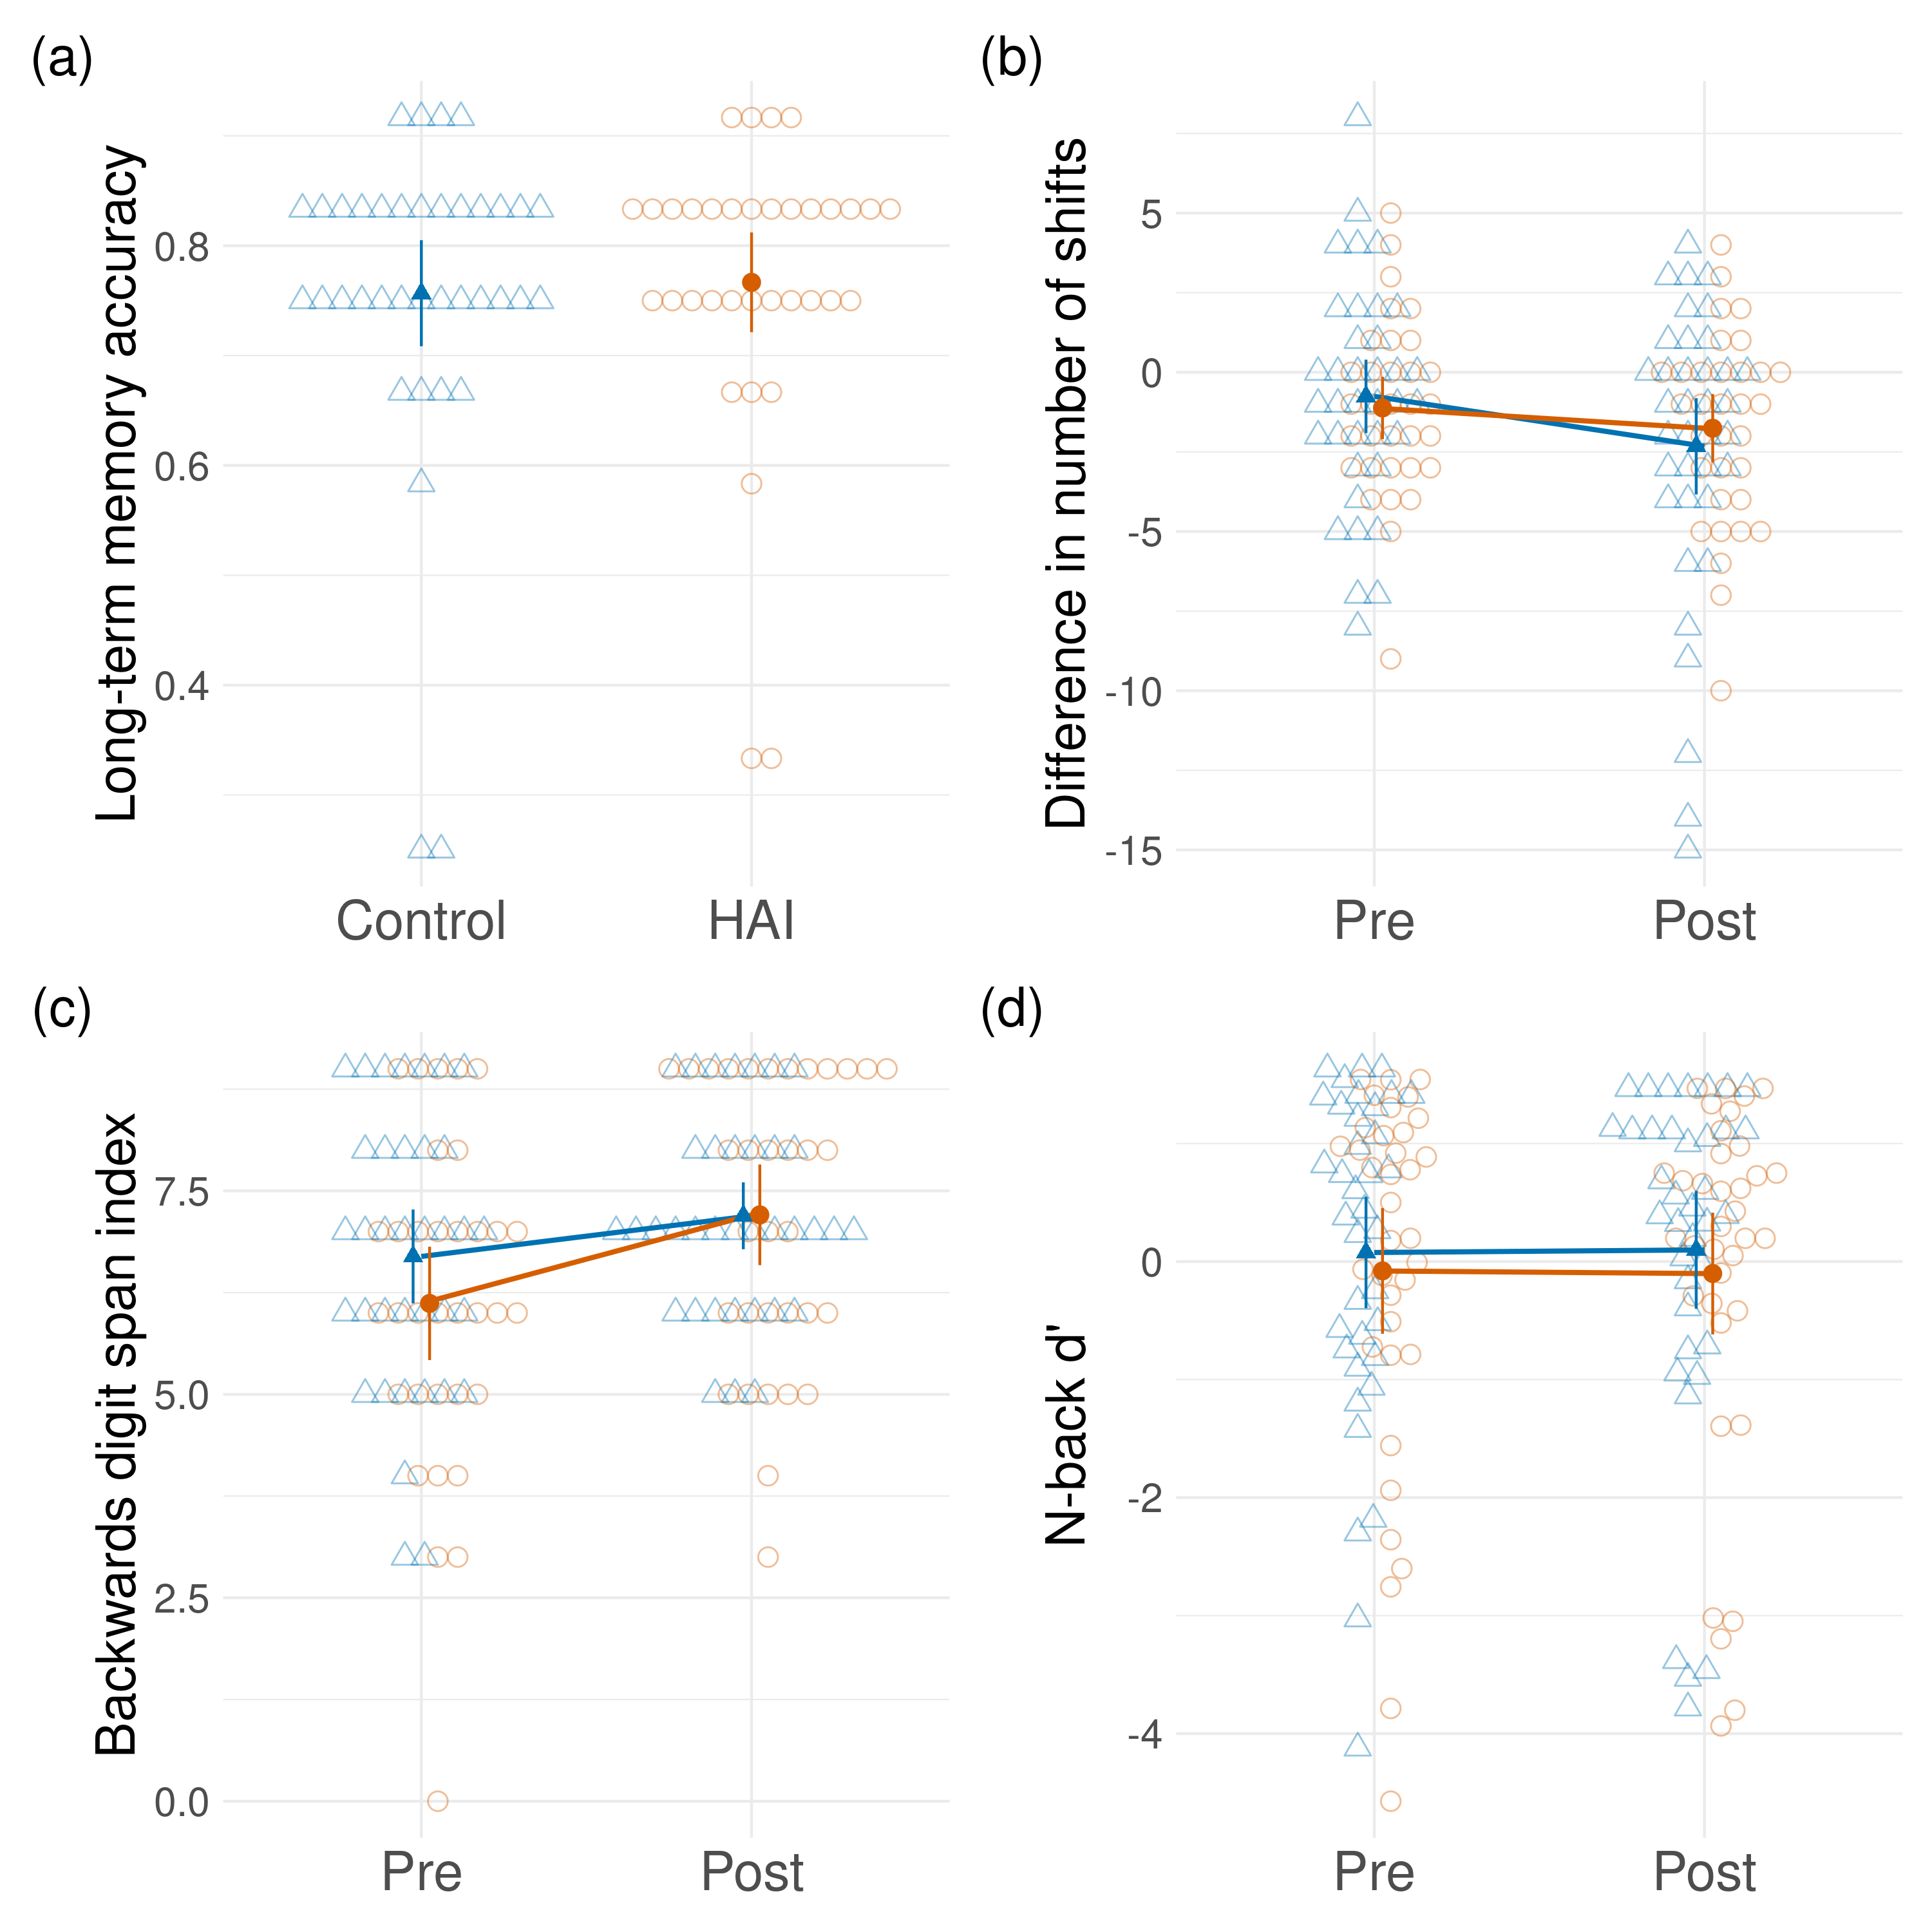
\includegraphics[width=0.9\linewidth]{/mnt/data/jstevens/OneDrive/active_sync/projects/haicognition2021/figures/cognitive_prepost_1} \caption{Cognitive performance for control and HAI (human-animal interaction) groups in Experiment 1. (a) Long-term memory accuracy from the Deese-Roedinger-McDermott task was calculated only post-condition. Pre- (Pre) and post-condition (Post) performance was calculated for (b) the difference in number of attentional shifts between the two Necker cube trials, (c) the index for the backwards digit span task, and (d) \(d'\) for the n-back task. Open triangles (blue) represent individual control participant scores, open circles (orange) represent individual HAI participant scores, closed triangles and circles represent condition group means (with lines connecting condition means), error bars represent 95\% confidence intervals.}\label{fig:cognitivea}
\end{figure*}

\hypertarget{exploratory-analyses}{%
\subsubsection{Exploratory analyses}\label{exploratory-analyses}}

We tested affect and pet attitude as potential moderators of the effect of HAI on cognition. There is substantial evidence to suggest that there were no observable moderators on the effect of experimental condition on composite cognitive performance. Specifically, the moderation model did not outperform an intercept-only model for positive affect change (\(R^2 = .01\), 90\% CI \([0.00\), \(0.04]\), \(F(3, 63) = 0.30\), \(p = .828\); \(BF\) = 0.04), negative affect change (\(R^2 = .02\), 90\% CI \([0.00\), \(0.06]\), \(F(3, 63) = 0.41\), \(p = .746\); \(BF\) = 0.04), or pet attitude (\(R^2 = .04\), 90\% CI \([0.00\), \(0.11]\), \(F(3, 63) = 0.86\), \(p = .468\); \(BF\) = 0.06).

We found that pet attitude positively correlated with the positive interaction quality measures from Gee et al. (2015) (comfort and desire to interact with the dog) and the change in positive PANAS between pre- and post-condition (Figure S4a), while negatively correlating with discomfort and ambivalence with the dog. The cognitive performance composite score did not correlate with any animal-related measures.

\hypertarget{summary-of-results}{%
\subsubsection{Summary of results}\label{summary-of-results}}

Our first investigation of the effects of HAI on affect and cognition replicated effects of HAI on affect but did not evoke predicted improvements in cognitive performance. Specifically, a three-minute animal interaction bolstered positive affect more so than a control activity. But we did not observe improvements in attentional control or working memory. Our follow-up moderation analyses indicated that affect and pet attitude did not moderate a relationship between experimental condition and cognitive performance.

\hypertarget{experiment-2}{%
\section{Experiment 2}\label{experiment-2}}

Our aim with Experiment 2 was to replicate Experiment 1 and extend the investigation to the influence of HAI on anxiety and stress. We assessed self-reports of anxiety and stress throughout the experiment using visual analogue scales. We again conducted follow-up exploratory analyses to identify potential moderators of the relationship between experimental condition and cognitive performance.

\hypertarget{methods-1}{%
\subsection{Methods}\label{methods-1}}

\hypertarget{participants-1}{%
\subsubsection{Participants}\label{participants-1}}

We recruited a new sample of participants between Nov 2018 to Apr 2019 from the University of Nebraska-Lincoln psychology subject pool who did not have a physical or emotional aversion to dogs (i.e., allergy, fear), again without providing information about dogs in the study description or consent materials. We analyzed data from 83 of 84 participants, excluding one person who progressed through the study without completing the experimental manipulation. Of the 83 eligible participants, 66 (79.5\%) identified as female, 17 (20.5\%) identified as male, and 0 (0.0\%) identified as neither male nor female (race/ethnicity and parental income information available in Table S1). Participants were on average 19.9 (\emph{SD} = 1.8) years of age (Table S1). There were 47 individuals (56.6\%) who currently live with at least one pet in their primary residence and 67 (80.7\%) who lived with at least one pet as a child. All participants received one hour of research credit in exchange for their participation.

\hypertarget{measures-1}{%
\subsubsection{Measures}\label{measures-1}}

In addition to the measures used in Experiment 1, we also explored the influence of human-animal interaction on affect through measures of anxiety and stress.

\textbf{\emph{Affect.}}
We assessed participants' present and general feelings of anxiety with the State and Trait Anxiety Inventory {[}STAI; Spielberger et al. (1999){]}. Participants were presented with 20 statements (e.g., ``I feel calm'') and rated each from one (\emph{not at all}) to four (\emph{very much so}) to describe their feelings in the moment (\emph{state}; \(\omega\) = 0.93), then rated another set of 20 to describe their feelings in general (\emph{trait}; \(\omega\) = 0.95). We also measured present feelings of anxiety with the single-item Anxiety Visual Analogue Scale {[}AVAS; Cella and Perry (1986){]}. Participants indicated how anxious they felt in the moment via mouse-click between poles \emph{not at all anxious} and \emph{extremely anxious} on a 100-tick horizontal line. Participants also indicated how stressed they felt in the moment with the similar Stress Visual Analogue Scale {[}SVAS; Cella and Perry (1986){]}. Higher values represent stronger feelings of anxiety and stress.

\textbf{\emph{Animal-related measures.}}
Participants responded to the same the animal-related measures used in Experiment 1, including the pet attitude scale (\(\omega\) = 0.93) and the HAI experience questions (\(\omega\) = 0.86). In addition, the researcher logged the amount of time the participant spent physically interacting with the dog, which ranged from 30 sec to the full 3 min.

\hypertarget{procedures-1}{%
\subsubsection{Procedures}\label{procedures-1}}

All procedures from Experiment 1 carried over to Experiment 2. However, instead of beginning with the Positive and Negative Affect Schedule, participants first completed Anxiety and Stress Visual Analogue Scales (\emph{baseline}), then STAI prior to PANAS. Participants also completed Visual Analogue Scales immediately preceding the 3-minute animal interaction/control condition (\emph{pre-condition} or \emph{pre}), immediately following the condition (\emph{post-condition} or \emph{post}), and following completion of the experiment (\emph{post+20}).

\hypertarget{analysis-1}{%
\subsubsection{Analysis}\label{analysis-1}}

Of the 83 eligible participants, 42 participants experienced the animal-interaction condition and 41 experienced the control condition. We increased our sample size slightly from Experiment 1 to boost power.

\textbf{\emph{Participant characteristics.}}
There were no between-group differences in pre-condition scores for any affective measures, cognitive tasks, or animal-related measures (Table \ref{tab:expt2scores}).

\textbf{\emph{Data analysis.}}
We utilized the same data analysis approach as Experiment 1 and also used this approach to analyze AVAS and SVAS (immediately before and after intervention). For moderation analyses, we tested all Experiment 1 moderators in addition to state and trait anxiety (from STAI), anxiety change from immediately pre- to post-condition (from AVAS), and stress change from immediately pre- to post-condition (from SVAS). We also included these additional measures in exploratory correlations between pet experience, affect, and cognition for those who experienced the animal interaction.

We log-transformed negative affect pre- and post-scores and removed a single outlier (standard deviation \(\times\) 3) to conform to analysis of covariance model assumptions. We excluded one observation from DRM (participant expressed comprehension issues after task), three from Necker cube (participants expressed comprehension issues after task), six from digit span (participants did not request response sheet or did not complete more than half of task), and three from n-back (two participants did not record any responses and one participant expressed comprehension issues after task).

\begin{table*}

\caption{\label{tab:expt2scores}Experiment 2 scores}
\centering
\resizebox{\linewidth}{!}{
\begin{threeparttable}
\begin{tabular}[t]{lrrrrrrrrrr}
\toprule
\multicolumn{1}{c}{} & \multicolumn{5}{c}{Pre-condition} & \multicolumn{5}{c}{Post-condition} \\
\cmidrule(l{3pt}r{3pt}){2-6} \cmidrule(l{3pt}r{3pt}){7-11}
Measure & $n$ & Control $M$ & HAI $M$ & $p$ & $BF$ & $n$ & Control $M$ & HAI $M$ & $p$ & $BF$\\
\midrule
\addlinespace[0.3em]
\multicolumn{11}{l}{\textbf{Pet measures}}\\
\hspace{1em}Pets now (\%) & -- & 60.98 & 52.38 & -- & -- & -- & -- & -- & -- & --\\
\hspace{1em}Pets as a child (\%) & -- & 82.93 & 78.57 & -- & -- & -- & -- & -- & -- & --\\
\hspace{1em}Pet attitude (PAS) & 83 & 5.84 & 5.90 & 0.67 & 0.18 & -- & -- & -- & -- & --\\
\addlinespace[0.3em]
\multicolumn{11}{l}{\textbf{Affective measures}}\\
\hspace{1em}Positive affect (PANAS) & 83 & 2.96 & 3.09 & 0.45 & 0.30 & 83 & 2.77 & 3.25 & < 0.001 & > 100\\
\hspace{1em}Negative affect (PANAS) & 83 & 1.44 & 1.40 & 0.96 & 0.17 & 82 & 0.25 & 0.13 & < 0.001 & 9.40\\
\hspace{1em}Anxiety (AVAS) & 83 & 28.83 & 36.45 & 0.11 & 0.63 & 83 & 23.28 & 14.28 & < 0.001 & 11.13\\
\hspace{1em}Stress (SVAS) & 83 & 33.73 & 39.36 & 0.18 & 0.33 & 83 & 25.44 & 17.12 & 0.01 & 3.03\\
\hspace{1em}State anxiety (STAI) & 83 & 36.22 & 34.00 & 0.25 & 0.34 & -- & -- & -- & -- & --\\
\hspace{1em}Trait anxiety (STAI) & 83 & 40.88 & 38.55 & 0.37 & 0.27 & -- & -- & -- & -- & --\\
\addlinespace[0.3em]
\multicolumn{11}{l}{\textbf{Cognitive tasks}}\\
\hspace{1em}Accuracy (DRM) & -- & -- & -- & -- & -- & 82 & 0.74 & 0.71 & 0.48 & 0.20\\
\hspace{1em}Average shifts (NCPC) & 80 & 0.15 & -1.15 & 0.19 & 0.35 & 80 & -1.51 & -1.93 & 0.52 & 0.28\\
\hspace{1em}Index (Digit span) & 77 & 5.84 & 6.13 & 0.43 & 0.21 & 77 & 6.83 & 6.52 & 0.39 & 0.32\\
\hspace{1em}$d'$ (N-back) & 80 & -0.09 & 0.30 & 0.19 & 0.49 & 80 & 0.00 & 0.11 & 0.61 & 0.26\\
\bottomrule
\end{tabular}
\begin{tablenotes}
\item \textit{Note: } 
\item Post-condition scores control for pre-condition scores.
\end{tablenotes}
\end{threeparttable}}
\end{table*}

\hypertarget{results-1}{%
\subsection{Results}\label{results-1}}

\hypertarget{affect-anxiety-and-stress}{%
\subsubsection{Affect, anxiety, and stress}\label{affect-anxiety-and-stress}}

Figures \ref{fig:panasb}a\&b demonstrate the effect of condition on positive and negative affect (Table \ref{tab:expt2scores}; Figure S5a\&b). As observed in Experiment 1, analysis of covariance revealed that there is very strong evidence that positive affect was greater post-condition for those who experienced the animal interaction than those who did not, controlling for pre-condition scores (\(F(1, 80) = 18.68\), \(\mathit{MSE} = 0.25\), \(p < .001\), \(\hat{\eta}^2_G = .189\), \(BF\) \textgreater{} 100). Contrary to Experiment 1, there is strong evidence that log negative affect was lower for those in the animal interaction group than the control group (\(F(1, 79) = 8.92\), \(\mathit{MSE} = 0.03\), \(p = .004\), \(\hat{\eta}^2_G = .102\), \(BF\) = 9.40).



\begin{figure*}
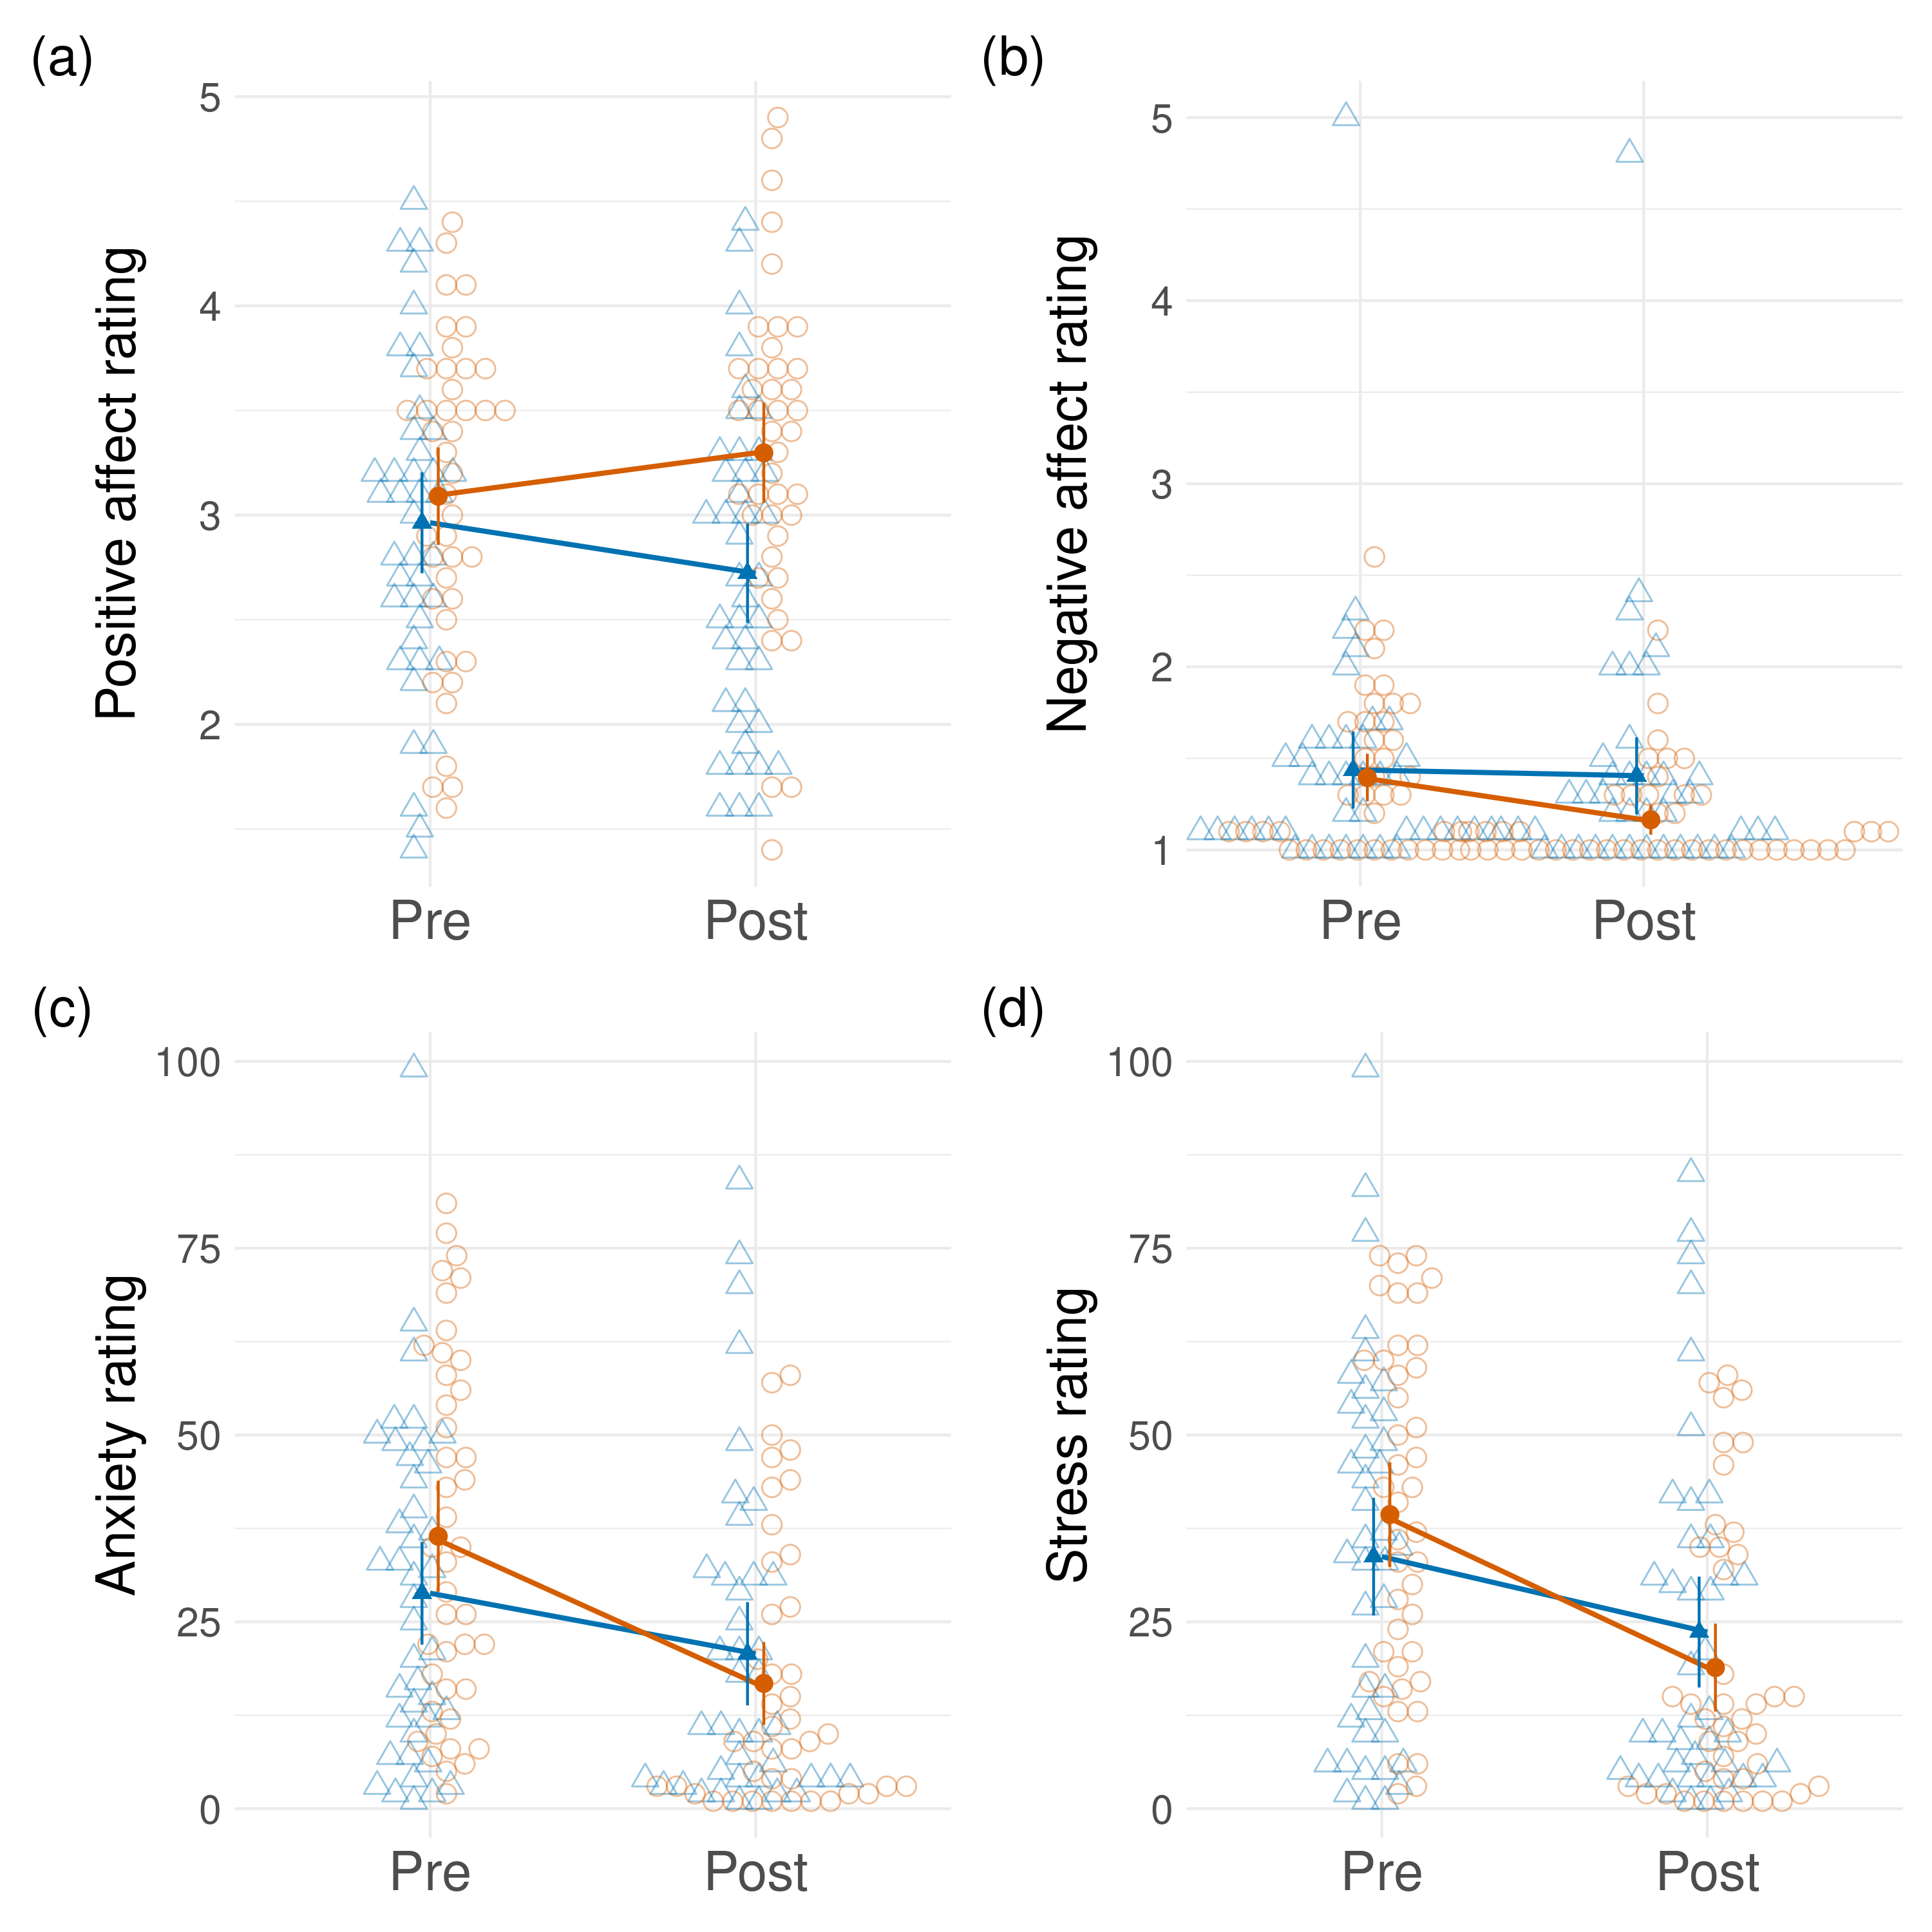
\includegraphics[width=0.9\linewidth]{/mnt/data/jstevens/OneDrive/active_sync/projects/haicognition2021/figures/affect_prepost_2} \caption{Affect scores pre- and post-condition for control and HAI (human-animal interaction) groups in Experiment 2. Scores show (a) positive PANAS ratings, (b) negative PANAS ratings, (c) anxiety ratings, and (d) stress ratings. Open triangles (blue) represent individual control participant scores, open circles (orange) represent individual HAI participant scores, closed triangles and circles represent condition group means (with lines connecting condition means), error bars represent 95\% confidence intervals.}\label{fig:panasb}
\end{figure*}

The effect of condition on anxiety and stress ratings is demonstrated by Figures \ref{fig:panasb}c\&d and S5c\&d and Table \ref{tab:expt2scores}. There is strong evidence that anxiety was lower post-condition for HAI compared to control (\(F(1, 80) = 9.50\), \(\mathit{MSE} = 172.00\), \(p = .003\), \(\hat{\eta}^2_G = .106\), \(BF\) = 11.13) and moderate evidence that stress was lower for those who experienced HAI than control (\(F(1, 80) = 6.20\), \(\mathit{MSE} = 228.68\), \(p = .015\), \(\hat{\eta}^2_G = .072\), \(BF\) = 3.03) when controlling for pre-condition scores.

\hypertarget{cognitive}{%
\subsubsection{Cognitive}\label{cognitive}}

There is no evidence to suggest that human-animal interaction and control groups differed on any measure of cognition (Table \ref{tab:expt2scores}; Figures \ref{fig:cognitiveb} and S6). Specifically, there is moderate evidence that there is no difference between control and HAI groups for the long-term memory task at post-condition (\(W = 767.00\), \(p = .485\), \(r\) = 0.08, \(BF\) = 0.20), the average switches in the Necker cube controlled attention task (\(F(1, 77) = 0.43\), \(\mathit{MSE} = 8.19\), \(p = .516\), \(\hat{\eta}^2_G = .005\), \(BF\) = 0.28), the n-back working memory task (\(F(1, 77) = 0.26\), \(\mathit{MSE} = 0.92\), \(p = .610\), \(\hat{\eta}^2_G = .003\), \(BF\) = 0.26), and the digit span working memory task (\(F(1, 74) = 0.76\), \(\mathit{MSE} = 2.42\), \(p = .385\), \(\hat{\eta}^2_G = .010\), \(BF\) = 0.32).



\begin{figure*}
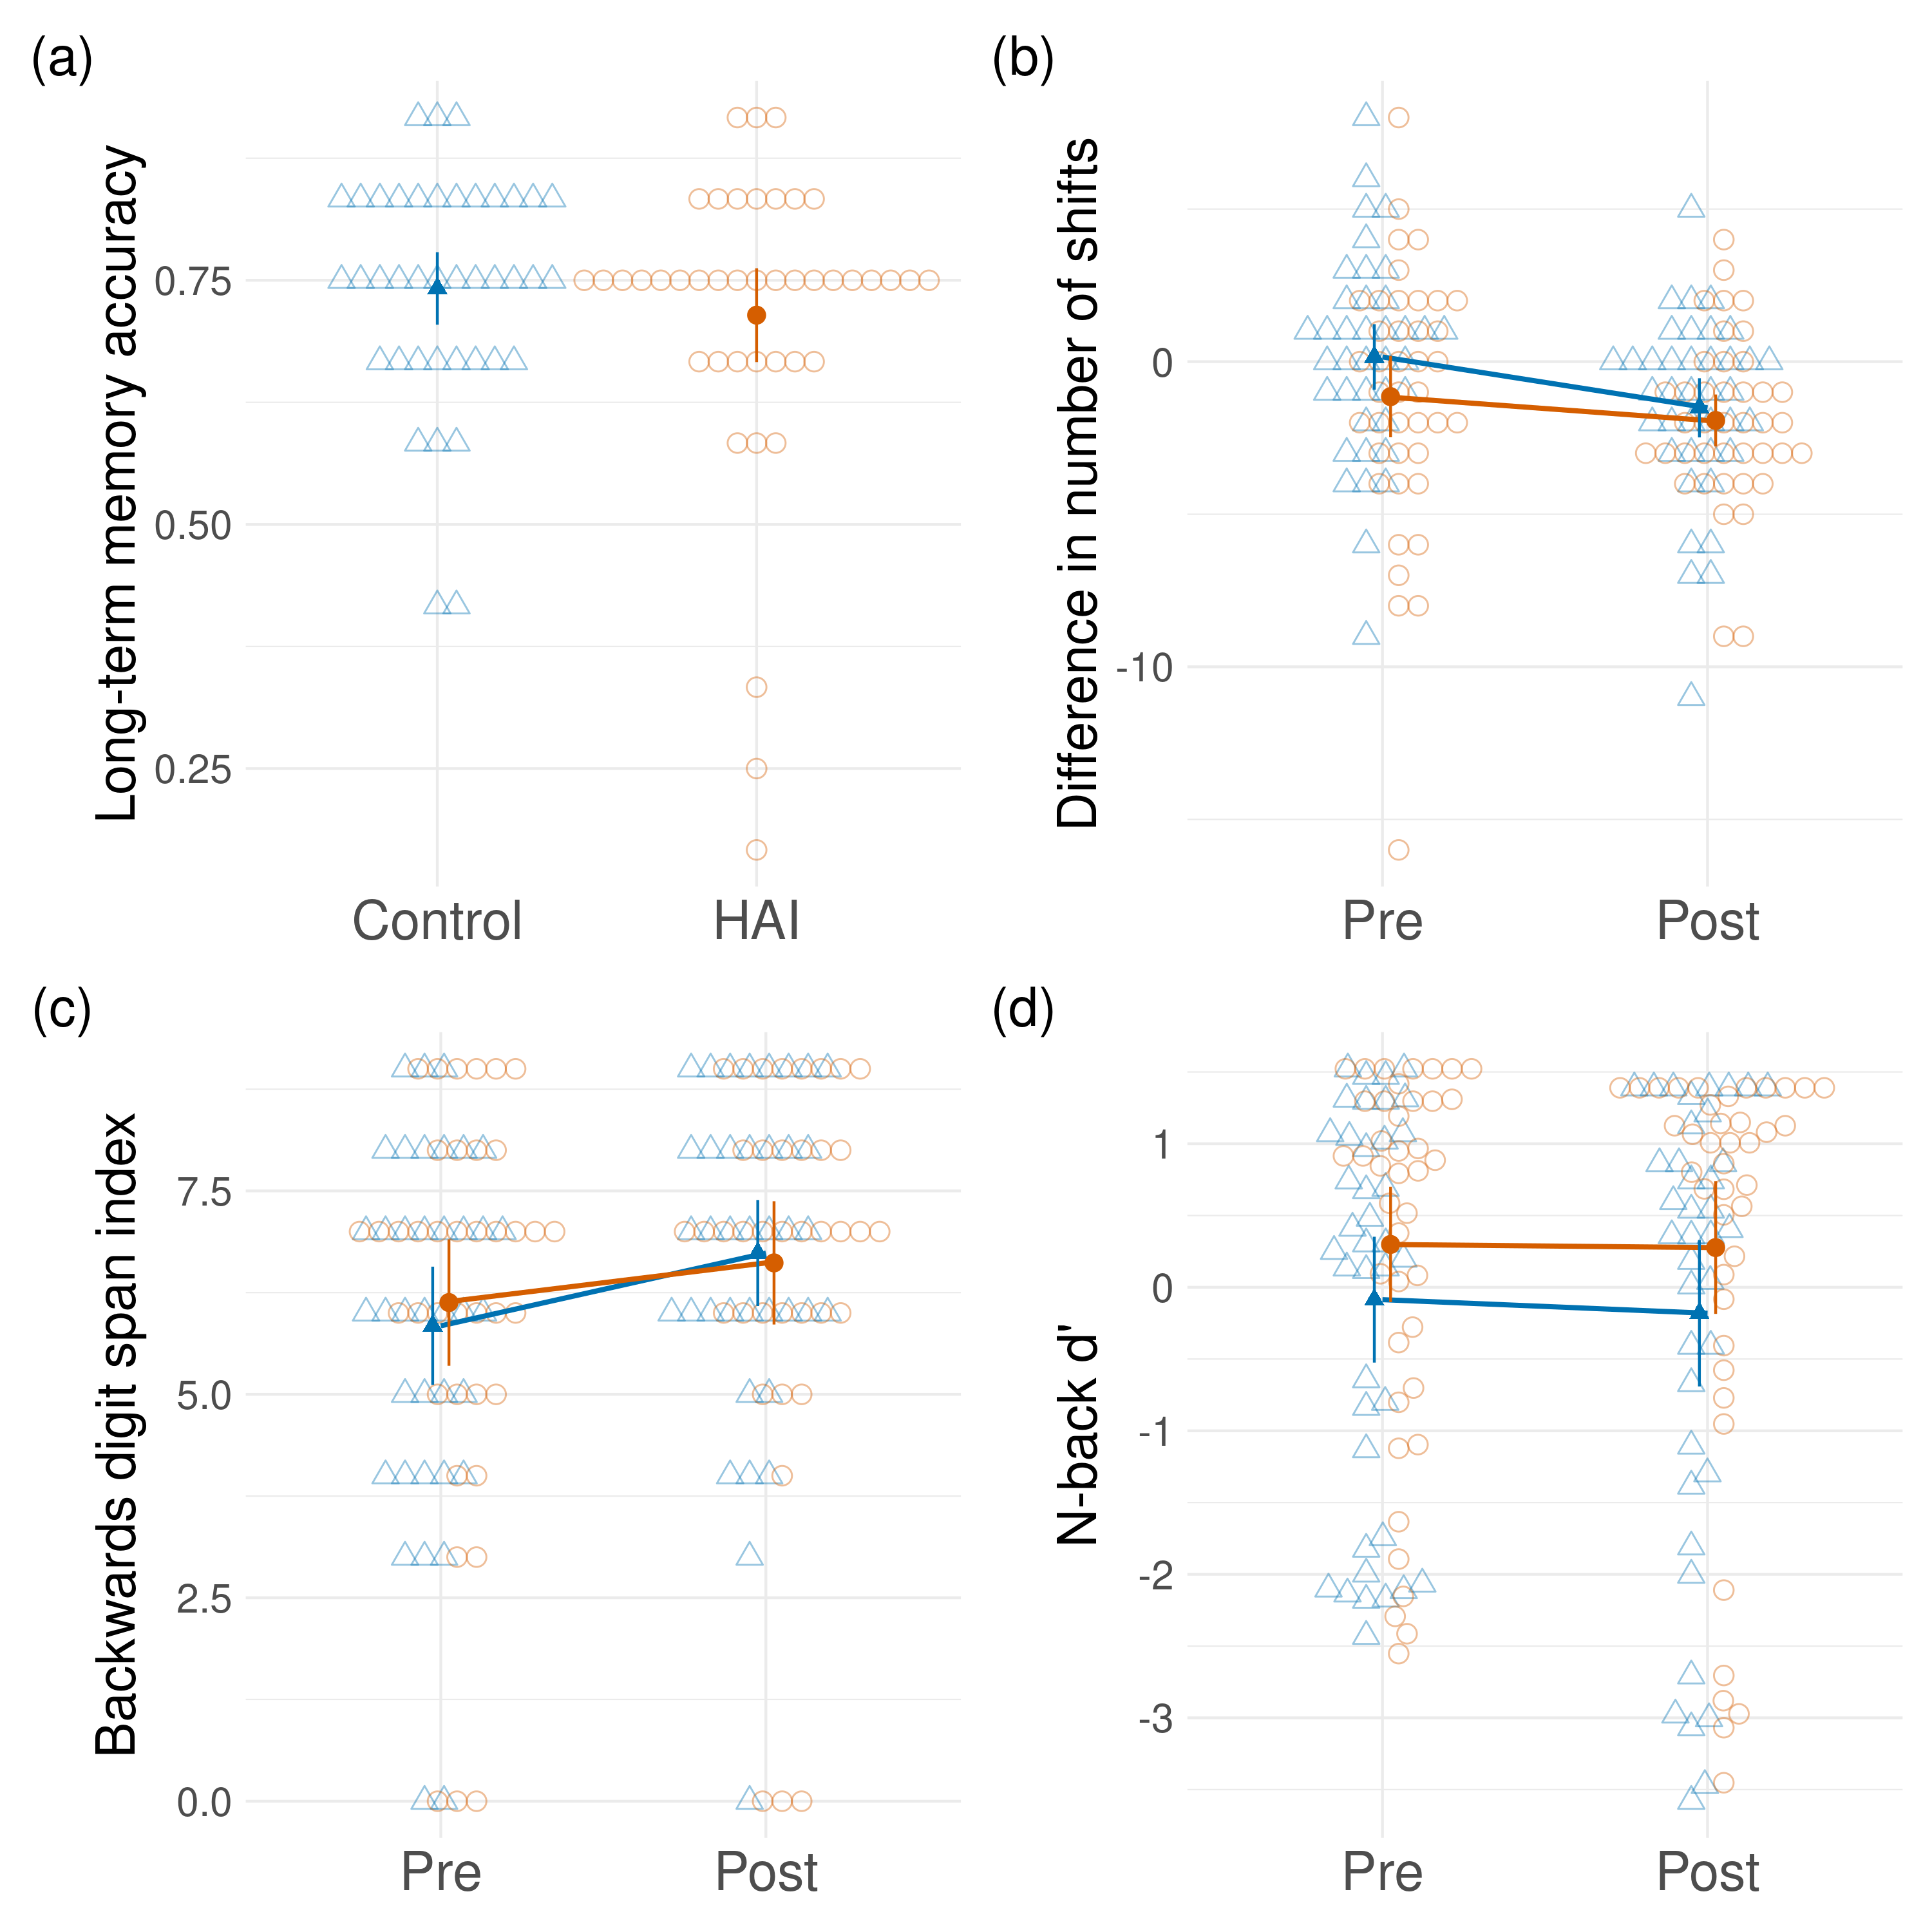
\includegraphics[width=0.9\linewidth]{/mnt/data/jstevens/OneDrive/active_sync/projects/haicognition2021/figures/cognitive_prepost_2} \caption{Cognitive performance for control and HAI (human-animal interaction) groups in Experiment 2. (a) Long-term memory accuracy from the Deese-Roedinger-McDermott task was calculated only post-condition. Pre- (Pre) and post-condition (Post) performance was calculated for (b) the difference in number of attentional shifts between the two Necker cube trials, (c) the index for the backwards digit span task, and (d) \(d'\) for the n-back task. Open triangles (blue) represent individual control participant scores, open circles (orange) represent individual HAI participant scores, closed triangles and circles represent condition group means (with lines connecting condition means), error bars represent 95\% confidence intervals.}\label{fig:cognitiveb}
\end{figure*}

\hypertarget{exploratory-analyses-1}{%
\subsubsection{Exploratory analyses}\label{exploratory-analyses-1}}

In line with Experiment 1, there is no evidence that the same variables nor the anxiety- and stress-related variables moderated the relationship between experimental condition and composite cognitive performance. Specifically, there is evidence that condition-cognition moderation models did not outperform intercept-only models for pet attitude (\(R^2 = < .01\), 90\% CI \([0.00\), \(1.00]\), \(F(3, 68) = 0.07\), \(p = .973\); \(BF\) = 0.02), positive affect change (\(R^2 = .05\), 90\% CI \([0.00\), \(0.12]\), \(F(3, 68) = 1.15\), \(p = .336\); \(BF\) = 0.08), negative affect change (\(R^2 = .03\), 90\% CI \([0.00\), \(0.08]\), \(F(3, 68) = 0.64\), \(p = .589\); \(BF\) = 0.05), stress change from pre- to post-condition (\(R^2 = .02\), 90\% CI \([0.00\), \(0.05]\), \(F(3, 68) = 0.36\), \(p = .781\); \(BF\) = 0.03), anxiety change from pre- to post-condition (\(R^2 = < .01\), 90\% CI \([0.00\), \(1.00]\), \(F(3, 68) = 0.06\), \(p = .979\); \(BF\) = 0.02), STAI-State anxiety (\(R^2 = .04\), 90\% CI \([0.00\), \(0.11]\), \(F(3, 68) = 1.02\), \(p = .390\); \(BF\) = 0.40), and STAI-Trait anxiety (\(R^2 = .04\), 90\% CI \([0.00\), \(0.11]\), \(F(3, 68) = 1.00\), \(p = .400\); \(BF\) = 0.07).

We replicated finding (1) positive relationships between pet attitude and comfort with the dog, desire to interact with the dog, and the change in positive PANAS, (2) negative relationships with discomfort and ambivalence with the dog, and (3) no relationships with cognitive performance composite (Figure S4b). Pet attitude also positively correlated with trait anxiety and negatively correlated with change in negative PANAS, feelings of stress, and feelings of anxiety.

\hypertarget{summary-of-results-1}{%
\subsubsection{Summary of results}\label{summary-of-results-1}}

Our findings from Experiment 2 provided nearly identical results to those we observed in Experiment 1. We observed once more that a three-minute HAI bolstered positive affect more so than a control; however, unlike in Experiment 1, HAI reduced negative affect. Further, human-animal interaction evoked lower stress and anxiety than the control. We did not observe differential improvements in attentional control or working memory between control and HAI groups. All follow-up moderation analyses mirrored those conducted in Experiment 1 such that affect change, ratings of anxiety and stress change, pet attitude, and state and trait anxiety did not influence the relationship between experimental condition and cognitive performance.

\hypertarget{discussion}{%
\section{Discussion}\label{discussion}}

Taken together, our findings provide support for the efficacy of animal interaction on affect but no evidence to suggest that animal interaction influences executive function. Specifically, there was greater positive affect improvement in HAI compared to control groups in both Experiments 1 and 2. Though we did not have evidence of effects of HAI on negative affect in Experiment 1, this likely resulted from a slightly smaller sample size. With the larger sample size of Experiment 2, we found that negative affect was reduced more in human-animal interaction than control groups. Anxiety and stress measures included in Experiment 2 captured more pronounced decreases in anxiety and stress for HAI compared to control groups. Nevertheless, measures of cognitive performance (long-term memory, working memory, and attentional control) did not differ between control and HAI groups in Experiments 1 or 2.

Improvements in affect following brief interactions with an unfamiliar animal are commonly observed in experimental HAI manipulations (Beetz et al., 2012; Lass-Hennemann et al., 2014; Crossman et al., 2015; Grajfoner et al., 2017), although future research should explore how long these effects last. Our evidence of a positive affect-boosting effect of animal interaction in both experiments validates our experimental design. We observed similar improvements in negative affect, anxiety, and stress in Experiment 2. Given the modest effect sizes observed here, three minutes may be a \emph{minimally} effective interaction period. In fact, a recent dose-response investigation found that low doses of HAI (i.e., three minutes) elicited stress improvement in a majority of participants but that \emph{maximal} improvement relative to time spent was reached with 15 minute doses (Fournier, 2019). Thus, longer interaction durations could induce changes in cognition not observed here. Note that this work focuses on the short-term interactions used in animal-assisted interventions. It is not clear whether they carry over into longer-term interactions associated with pet ownership.

Given the evidence that HAI influences affect and stress, which in turn can influence cognition, we expected HAI to influence cognition. In particular, we expected HAI to influence executive functioning because HAI shares characteristics with another literature---exposure to natural landscapes---that does influence attentional control and working memory. Because animals are an inherent part of nature, and HAI has been tied to biophilia as well, the nature exposure literature created a conceptual framework for predicting that HAI could influence executive functioning. However, our results---and the results of others (Gee et al., 2014, 2015; Hediger \& Turner, 2014; Trammell, 2019)---run counter to the findings in the exposure to nature literature.

There are at least two possible reasons why our results do not follow the findings in the nature exposure literature. First, there may just be a fundamental difference between exposure to nature and interacting with animals. Perhaps biophilia may elicit strong affective effects in both nature and animal interactions because they share a similar experiential component. However, the improvement in affect triggers downstream effects on cognition differently with animals and nature. Similarly, cognitive restoration observed following experiences in nature may not be attributable to biophilia alone because these effects are dependent on aesthetic features unique to natural environments, whereby cognitive improvement is facilitated by a more complex mechanism. Also, using biophilia as the framework connecting the nature exposure literature with human-animal interaction may not be as clear-cut as would be expected. While early work suggested that animal interactions should fit within the biophilia framework (Lawrence, 1993), more recent critiques suggests a more nuanced approach (Joye \& De Block, 2011). For example, observed HAI effects on well-being may be due to the calming and supernormal stimulus properties of animals or social/cultural effects rather than them being historically important in our evolution (Serpell, 2004; Kruger \& Serpell, 2010). Even within an evolutionary framework, animals typically fall into categories of predator or prey, and we may have evolved specific cognition to avoid predators and capture prey (Barrett, 2015). From this perspective, some species are functional in terms of consuming their meat, whereas others are to be feared and avoided. This view would predict differences between species, with predator species probably not enhancing well-being to the degree that less threatening species might. Thus, human-animal relationships are not as straightforward as proposed in the original biophilia hypothesis, and this hypothesis may not have strong predictions about how interacting with animals should influence human well-being.

An alternative possibility is that our experimental paradigm did not trigger latent cognitive effects of HAI. Perhaps exposure to nature can reach the threshold for triggering these effects easily, but the threshold is higher or harder to reach for animal interactions. Or the time lag for these effects may be delayed (e.g., Handlin et al., 2011). Thus, experimental design could be critical for studying HAI effects on cognition. Decisions about durations of exposure, number and timing of cognitive tasks, and the presence of stress induction could be important in eliciting effects of animal interactions (Fournier, 2019; Griffin et al., 2019), as has been demonstrated in the exposure to nature literature (Shanahan et al., 2016; Cox et al., 2017; Stevenson et al., 2018; Stenfors et al., 2019).

Alternatively, other factors could moderate potential HAI effects on cognition. Individual and cultural differences in interactions with animals can moderate effects on well-being (Barker et al., 2010) and could potentially moderate effects on cognition. This possibility necessitates inclusion of individual difference measures, such as pet attitudes, to better understand the factors influencing potential HAI effects on cognition. Though we found no moderating effect of pet attitudes or ownership in our analysis, these types of factors are important to help profile individuals and groups best suited for animal interventions (Melson, 2011; McCune et al., 2014, 2020).

Thus far in the field, the experimental design attributes of human-animal interaction delivery, duration, and features have been a function of convenience and guesswork as opposed to driven by theory. The field is in need of a grounding framework to systematically grow this understanding. The neighboring domain of exposure to nature literature may provide a suitable, rigorously studied foundation (Kaplan \& Berman, 2010; Bratman et al., 2012; Schertz \& Berman, 2019). By taking advantage of the affective and cognitive frameworks embedded within the exposure to nature literature, HAI practitioners provide themselves with the chance to standardize investigations of cognitive performance and draw theoretically sound inferences from their findings. Evidence of this sort is well-positioned to inform decisions regarding the implementation of HAIs in schools and other performance-dependent contexts for healthy and clinical populations. A deeper understanding of the influence of HAIs on cognition can also provide necessary footing to investigate whether observations are moderated by life experiences, such as growing up in an urban or rural community, race/ethnicity, socio-economic status, or personal history with animals. With affiliative animals like dogs so accessible in daily life, it is crucial to profile the restorative potential of these therapeutic agents by furthering research into the influence of animal interactions on cognition.

Our study investigated HAI in student participants and replicated effects on affect (Stewart et al., 2014; Crossman et al., 2015; Crump \& Derting, 2015) and lack of effects on cognition (Gee et al., 2014, 2015; Trammell, 2019) observed in similar populations. Undergraduate students are a unique and unrepresentative population, potentially limiting the application of these findings to other populations. Nevertheless, the high levels of stress and anxiety experienced by students---and the pressure for high levels of cognitive performance---underscore the importance of understanding these effects in this population. Furthermore, the effect of HAI on affect (Crossman et al., 2020) and and the lack of an effect on cognition (Hediger \& Turner, 2014) has also been documented in children, suggesting that our findings may generalize beyond undergraduate students. Yet even the sample of undergraduates that we tested is not representative, with a bias toward female, white, affluent participants who owned pets as children. Further research must assess if these findings generalize to other populations.

In addition to a potentially unrepresentative sample of participants, the experimental design may have imposed limitations on the ecological validity of the study. The controlled nature of the experimental setting may have inhibited participants from engaging with the dog in a natural way. Participants may have found having the experimenter in the room or the admonition to avoiding `riling up' the dog to be awkward for engaging in a natural interaction. Thus, differently structured interactions (e.g., in less prescribed or group settings) could result in different outcomes.

Experimental outcomes could also depend on how familiar participants are with the dogs. People interacting with their own dog or a familiar dog may have a more enjoyable experience, which may put them in a different state of mind for completing the cognitive tasks. Not knowing the dog may have made the participants more inhibited, precluding them from fully experiencing any possible benefits in cognitive performance.

\hypertarget{conclusion}{%
\subsection{Conclusion}\label{conclusion}}

In the present study, we addressed a need to strengthen theory-driven tests of the influence of human-animal interaction on cognition. We observed positive effects of HAI in affective measures---including positive affect, negative affect, anxiety, and stress---but did not observe improvement in cognitive performance. Future research should continue to enhance the connection between nature exposure and human-animal interaction studies to build our understanding of cognition in response to animal interactions.

\hypertarget{acknowledgments}{%
\section{Acknowledgments}\label{acknowledgments}}

We thank Megan Bosworth, Kendall Kelly, and Maggie Kempf for assistance in collecting the data and Francine Goh and London Wolff for comments on a previous draft. We dedicate this work to the memory of Koda, who made the project possible and a joy at every turn.

\hypertarget{conflict-of-interest}{%
\section{Conflict of interest}\label{conflict-of-interest}}

The authors declare no conflicts of interest.

\hypertarget{references}{%
\section*{References}\label{references}}
\addcontentsline{toc}{section}{References}

\hypertarget{refs}{}
\begin{CSLReferences}{1}{0}
\leavevmode\hypertarget{ref-R-papaja}{}%
Aust, F., \& Barth, M. (2020). \emph{{papaja}: {Create} {APA} manuscripts with {R Markdown}}. \url{https://github.com/crsh/papaja}

\leavevmode\hypertarget{ref-Barker.etal.2016}{}%
Barker, S. B., Barker, R. T., McCain, N. L., \& Schubert, C. M. (2016). A randomized cross-over exploratory study of the effect of visiting therapy dogs on college student stress before final exams. \emph{Anthrozoös}, \emph{29}(1), 35--46. \url{https://doi.org/10.1080/08927936.2015.1069988}

\leavevmode\hypertarget{ref-Barker.etal.2010}{}%
Barker, S. B., Knisely, J. S., McCain, N. L., Schubert, C. M., \& Pandurangi, A. K. (2010). Exploratory study of stress-buffering response patterns from interaction with a therapy dog. \emph{Anthrozoös}, \emph{23}(1), 79--91. \url{https://doi.org/10.2752/175303710X12627079939341}

\leavevmode\hypertarget{ref-Barker.etal.2003}{}%
Barker, S. B., Pandurangi, A. K., \& Best, A. M. (2003). Effects of animal-assisted therapy on patients' anxiety, fear, and depression before {ECT}. \emph{The Journal of ECT}, \emph{19}(1), 38. \url{https://doi.org/10.1097/00124509-200303000-00008}

\leavevmode\hypertarget{ref-Barker.Wolen.2008}{}%
Barker, S. B., \& Wolen, A. R. (2008). The benefits of human-companion animal interaction: {A} review. \emph{Journal of Veterinary Medical Education}, \emph{35}(4), 487--495. \url{https://doi.org/10.3138/jvme.35.4.487}

\leavevmode\hypertarget{ref-Barrett.2015}{}%
Barrett, H. C. (2015). Adaptations to predators and prey. In \emph{The {Handbook} of {Evolutionary Psychology}} (pp. 200--223). {John Wiley \& Sons, Ltd}. \url{https://doi.org/10.1002/9780470939376.ch7}

\leavevmode\hypertarget{ref-Beetz.2017}{}%
Beetz, A. M. (2017). Theories and possible processes of action in animal assisted interventions. \emph{Applied Developmental Science}, \emph{21}(2), 139--149. \url{https://doi.org/10.1080/10888691.2016.1262263}

\leavevmode\hypertarget{ref-Beetz.etal.2012}{}%
Beetz, A., Uvnäs-Moberg, K., Julius, H., \& Kotrschal, K. (2012). Psychosocial and psychophysiological effects of human-animal interactions: {The} possible role of oxytocin. \emph{Frontiers in Psychology}, \emph{3}, 234. \url{https://doi.org/10.3389/fpsyg.2012.00234}

\leavevmode\hypertarget{ref-Berman.etal.2008}{}%
Berman, M. G., Jonides, J., \& Kaplan, S. (2008). The cognitive benefits of interacting with nature. \emph{Psychological Science}, \emph{19}(12), 1207--1212. \url{https://doi.org/10.1111/j.1467-9280.2008.02225.x}

\leavevmode\hypertarget{ref-Bratman.etal.2015}{}%
Bratman, G. N., Daily, G. C., Levy, B. J., \& Gross, J. J. (2015). The benefits of nature experience: {Improved} affect and cognition. \emph{Landscape and Urban Planning}, \emph{138}, 41--50. \url{https://doi.org/10.1016/j.landurbplan.2015.02.005}

\leavevmode\hypertarget{ref-Bratman.etal.2012}{}%
Bratman, G. N., Hamilton, J. P., \& Daily, G. C. (2012). The impacts of nature experience on human cognitive function and mental health. \emph{Annals of the New York Academy of Sciences}, \emph{1249}(1), 118--136. \url{https://doi.org/10.1111/j.1749-6632.2011.06400.x}

\leavevmode\hypertarget{ref-Cadavid.Beato.2016}{}%
Cadavid, S., \& Beato, M. S. (2016). Memory distortion and its avoidance: {An} event-related potentials study on false recognition and correct rejection. \emph{PLOS ONE}, \emph{11}(10), e0164024. \url{https://doi.org/10.1371/journal.pone.0164024}

\leavevmode\hypertarget{ref-Cella.Perry.1986}{}%
Cella, D. F., \& Perry, S. W. (1986). Reliability and concurrent validity of three visual-analogue mood scales. \emph{Psychological Reports}, \emph{59}(2), 827--833. \url{https://doi.org/10.2466/pr0.1986.59.2.827}

\leavevmode\hypertarget{ref-Cimprich.1993}{}%
Cimprich, B. (1993). Development of an intervention to restore attention in cancer patients. \emph{Cancer Nursing}, \emph{16}(2), 83--92.

\leavevmode\hypertarget{ref-R-ggbeeswarm}{}%
Clarke, E., \& Sherrill-Mix, S. (2017). \emph{{ggbeeswarm}: Categorical scatter (violin point) plots}. \url{https://CRAN.R-project.org/package=ggbeeswarm}

\leavevmode\hypertarget{ref-Cohen.etal.1994}{}%
Cohen, J. D., Forman, S. D., Braver, T. S., Casey, B. J., Servan-Schreiber, D., \& Noll, D. C. (1994). Activation of the prefrontal cortex in a nonspatial working memory task with functional {MRI}. \emph{Human Brain Mapping}, \emph{1}(4), 293--304. \url{https://doi.org/10.1002/hbm.460010407}

\leavevmode\hypertarget{ref-Cox.etal.2017}{}%
Cox, D. T. C., Shanahan, D. F., Hudson, H. L., Fuller, R. A., Anderson, K., Hancock, S., \& Gaston, K. J. (2017). Doses of nearby nature simultaneously associated with multiple health benefits. \emph{International Journal of Environmental Research and Public Health}, \emph{14}(2), 172. \url{https://doi.org/10.3390/ijerph14020172}

\leavevmode\hypertarget{ref-Crossman.etal.2015}{}%
Crossman, M. K., Kazdin, A. E., \& Knudson, K. (2015). Brief unstructured interaction with a dog reduces distress. \emph{Anthrozoös}, \emph{28}(4), 649--659. \url{https://doi.org/10.1080/08927936.2015.1070008}

\leavevmode\hypertarget{ref-Crossman.etal.2020}{}%
Crossman, M. K., Kazdin, A. E., Matijczak, A., Kitt, E. R., \& Santos, L. R. (2020). The influence of interactions with dogs on affect, anxiety, and arousal in children. \emph{Journal of Clinical Child \& Adolescent Psychology}, \emph{49}(4), 535--548. \url{https://doi.org/10.1080/15374416.2018.1520119}

\leavevmode\hypertarget{ref-Crump.Derting.2015}{}%
Crump, C., \& Derting, T. L. (2015). Effects of pet therapy on the psychological and physiological stress levels of first-year female undergraduates. \emph{North American Journal of Psychology}, \emph{17}(3), 575.

\leavevmode\hypertarget{ref-Ein.etal.2018}{}%
Ein, N., Li, L., \& Vickers, K. (2018). The effect of pet therapy on the physiological and subjective stress response: {A} meta-analysis. \emph{Stress and Health}, \emph{34}(4), 477--489. \url{https://doi.org/10.1002/smi.2812}

\leavevmode\hypertarget{ref-Empatica.2018}{}%
Empatica. (2018). \emph{E4 {Wristband User}'s {Manual}}.

\leavevmode\hypertarget{ref-Fiocco.Hunse.2017}{}%
Fiocco, A. J., \& Hunse, A. M. (2017). The buffer effect of therapy dog exposure on stress reactivity in undergraduate students. \emph{International Journal of Environmental Research and Public Health}, \emph{14}(7), 707. \url{https://doi.org/10.3390/ijerph14070707}

\leavevmode\hypertarget{ref-Fournier.2019}{}%
Fournier, A. K. (2019). {HAI} dose in animal-assisted intervention. In A. K. Fournier (Ed.), \emph{Animal-{Assisted Intervention}: {Thinking Empirically}} (pp. 31--51). {Springer International Publishing}. \url{https://doi.org/10.1007/978-3-030-32972-3_3}

\leavevmode\hypertarget{ref-Franco.etal.2017}{}%
Franco, L. S., Shanahan, D. F., \& Fuller, R. A. (2017). A review of the benefits of nature experiences: {More} than meets the eye. \emph{International Journal of Environmental Research and Public Health}, \emph{14}(8), 864. \url{https://doi.org/10.3390/ijerph14080864}

\leavevmode\hypertarget{ref-Friedmann.Son.2009}{}%
Friedmann, E., \& Son, H. (2009). The human-companion animal bond: {How} humans benefit. \emph{Veterinary Clinics of North America: Small Animal Practice}, \emph{39}(2), 293--326. \url{https://doi.org/10.1016/j.cvsm.2008.10.015}

\leavevmode\hypertarget{ref-Gee.etal.2012}{}%
Gee, N. R., Belcher, J. M., Grabski, J. L., DeJesus, M., \& Riley, W. (2012). The presence of a therapy dog results in improved object recognition performance in preschool children. \emph{Anthrozoös}, \emph{25}(3), 289--300. \url{https://doi.org/10.2752/175303712X13403555186172}

\leavevmode\hypertarget{ref-Gee.etal.2010}{}%
Gee, N. R., Church, M. T., \& Altobelli, C. L. (2010). Preschoolers make fewer errors on an object categorization task in the presence of a dog. \emph{Anthrozoös}, \emph{23}(3), 223--230. \url{https://doi.org/10.2752/175303710X12750451258896}

\leavevmode\hypertarget{ref-Gee.etal.2017b}{}%
Gee, N. R., Fine, A. H., \& McCardle, P. (2017). Companion animals as moderators of stress responses: Implications for academic performance, testing, and achievement. In N. R. Gee \& E. Friedmann (Eds.), \emph{How {Animals Help Students Learn}: {Research} and {Practice} for {Educators} and {Mental}-{Health Professionals}} (pp. 120--132). {Taylor \& Francis}.

\leavevmode\hypertarget{ref-Gee.etal.2015}{}%
Gee, N. R., Fine, A. H., \& Schuck, S. (2015). Animals in educational settings: {Research} and practice. In A. H. Fine (Ed.), \emph{Handbook on {Animal}-{Assisted Therapy}} (Fourth, pp. 195--210). {Academic Press}. \url{https://doi.org/10.1016/B978-0-12-801292-5.00014-6}

\leavevmode\hypertarget{ref-Gee.etal.2014}{}%
Gee, N. R., Friedmann, E., Stendahl, M., Fisk, A., \& Coglitore, V. (2014). Heart rate variability during a working memory task: {Does} touching a dog or person affect the response? \emph{Anthrozoös}, \emph{27}(4), 513--528. \url{https://doi.org/10.2752/089279314X14072268687763}

\leavevmode\hypertarget{ref-Gidlow.etal.2016}{}%
Gidlow, C. J., Jones, M. V., Hurst, G., Masterson, D., Clark-Carter, D., Tarvainen, M. P., Smith, G., \& Nieuwenhuijsen, M. (2016). Where to put your best foot forward: {Psycho}-physiological responses to walking in natural and urban environments. \emph{Journal of Environmental Psychology}, \emph{45}, 22--29. \url{https://doi.org/10.1016/j.jenvp.2015.11.003}

\leavevmode\hypertarget{ref-Grajfoner.etal.2017}{}%
Grajfoner, D., Harte, E., Potter, L. M., \& McGuigan, N. (2017). The effect of dog-assisted intervention on student well-being, mood, and anxiety. \emph{International Journal of Environmental Research and Public Health}, \emph{14}(5), 483. \url{https://doi.org/10.3390/ijerph14050483}

\leavevmode\hypertarget{ref-Griffin.etal.2019}{}%
Griffin, J. A., Hurley, K., \& McCune, S. (2019). Human-animal interaction research: {Progress} and possibilities. \emph{Frontiers in Psychology}, \emph{10}, 2803. \url{https://doi.org/10.3389/fpsyg.2019.02803}

\leavevmode\hypertarget{ref-Haatveit.etal.2010}{}%
Haatveit, B. C., Sundet, K., Hugdahl, K., Ueland, T., Melle, I., \& Andreassen, O. A. (2010). The validity of d prime as a working memory index: {Results} from the {``{Bergen} n-back task.''} \emph{Journal of Clinical and Experimental Neuropsychology}, \emph{32}(8), 871--880. \url{https://doi.org/10.1080/13803391003596421}

\leavevmode\hypertarget{ref-Handlin.etal.2011}{}%
Handlin, L., Hydbring-Sandberg, E., Nilsson, A., Ejdebäck, M., Jansson, A., \& Uvnäs-Moberg, K. (2011). Short-term interaction between dogs and their owners: Effects on oxytocin, cortisol, insulin and heart rate---an exploratory study. \emph{Anthrozoös}, \emph{24}(3), 301--315. \url{https://doi.org/10.2752/175303711X13045914865385}

\leavevmode\hypertarget{ref-R-Hmisc}{}%
Harrell Jr, F. E., Charles Dupont, with contributions from, \& others., many. (2020). \emph{Hmisc: Harrell miscellaneous}. \url{https://CRAN.R-project.org/package=Hmisc}

\leavevmode\hypertarget{ref-Hediger.Turner.2014}{}%
Hediger, K., \& Turner, D. C. (2014). Can dogs increase children's attention and concentration performance? {A} randomised controlled trial. \emph{Human Animal Interaction Bulletin}, \emph{2}, 21--39.

\leavevmode\hypertarget{ref-Hosey.Melfi.2014}{}%
Hosey, G., \& Melfi, V. (2014). Human-animal interactions, relationships and bonds: A review and analysis of the literature. \emph{International Journal of Comparative Psychology}, \emph{27}(1).

\leavevmode\hypertarget{ref-Johnson.etal.2008a}{}%
Johnson, R. A., Meadows, R. L., Haubner, J. S., \& Sevedge, K. (2008). Animal-assisted activity among patients with cancer: Effects on mood, fatigue, self-perceived health, and sense of coherence. \emph{Oncology Nursing Forum}, \emph{35}(2), 225--232. \url{https://doi.org/10.1188/08.ONF.225-232}

\leavevmode\hypertarget{ref-Johnson.2016}{}%
Johnson, T. R. (2016). Violation of the homogeneity of regression slopes assumption in {ANCOVA} for two-group pre-post designs: {Tutorial} on a modified {Johnson}-{Neyman} procedure. \emph{The Quantitative Methods for Psychology}, \emph{12}(3), 253--263. \url{https://doi.org/10.20982/tqmp.12.3.p253}

\leavevmode\hypertarget{ref-Joye.DeBlock.2011}{}%
Joye, Y., \& De Block, A. (2011). {`{Nature} and {I} are two'}: {A} critical examination of the biophilia hypothesis. \emph{Environmental Values}, \emph{20}(2), 189--215.

\leavevmode\hypertarget{ref-Kane.etal.2007}{}%
Kane, M. J., Conway, A. R. A., Miura, T. K., \& Colflesh, G. J. H. (2007). Working memory, attention control, and the {N}-back task: A question of construct validity. \emph{Journal of Experimental Psychology. Learning, Memory, and Cognition}, \emph{33}(3), 615--622. \url{https://doi.org/10.1037/0278-7393.33.3.615}

\leavevmode\hypertarget{ref-Kaplan.Kaplan.1989}{}%
Kaplan, R., \& Kaplan, S. (1989). \emph{The {Experience} of {Nature}: {A Psychological Perspective}}. {Cambridge University Press}.

\leavevmode\hypertarget{ref-Kaplan.1995}{}%
Kaplan, S. (1995). The restorative benefits of nature: {Toward} an integrative framework. \emph{Journal of Environmental Psychology}, \emph{15}(3), 169--182. \url{https://doi.org/10.1016/0272-4944(95)90001-2}

\leavevmode\hypertarget{ref-Kaplan.Berman.2010}{}%
Kaplan, S., \& Berman, M. G. (2010). Directed attention as a common resource for executive functioning and self-regulation. \emph{Perspectives on Psychological Science}, \emph{5}(1), 43--57. \url{https://doi.org/10.1177/1745691609356784}

\leavevmode\hypertarget{ref-R-ggcorrplot}{}%
Kassambara, A. (2019). \emph{{ggcorrplot}: Visualization of a correlation matrix using {`ggplot2'}}. \url{https://CRAN.R-project.org/package=ggcorrplot}

\leavevmode\hypertarget{ref-Kruger.Serpell.2010}{}%
Kruger, K. A., \& Serpell, J. A. (2010). Animal-assisted interventions in mental health: Definitions and theoretical foundations. In A. H. Fine (Ed.), \emph{Handbook on {Animal}-{Assisted Therapy} ({Third Edition})} (pp. 33--48). {Academic Press}. \url{https://doi.org/10.1016/B978-0-12-381453-1.10003-0}

\leavevmode\hypertarget{ref-Lass-Hennemann.etal.2014}{}%
Lass-Hennemann, J., Peyk, P., Streb, M., Holz, E., \& Michael, T. (2014). Presence of a dog reduces subjective but not physiological stress responses to an analog trauma. \emph{Frontiers in Psychology}, \emph{5}, 1010. \url{https://doi.org/10.3389/fpsyg.2014.01010}

\leavevmode\hypertarget{ref-Lawrence.1993}{}%
Lawrence, E. A. (1993). The sacred bee, the filthy pig, and the bat out of hell: {Animal} symbolism as cognitive biophilia. In S. R. Kellert \& W. E. O. (Eds.), \emph{The Biophilia Hypothesis} (pp. 301--344). {Island Press}.

\leavevmode\hypertarget{ref-Li.Sullivan.2016}{}%
Li, D., \& Sullivan, W. C. (2016). Impact of views to school landscapes on recovery from stress and mental fatigue. \emph{Landscape and Urban Planning}, \emph{148}, 149--158. \url{https://doi.org/10.1016/j.landurbplan.2015.12.015}

\leavevmode\hypertarget{ref-MacDuffie.etal.2012}{}%
MacDuffie, K. E., Atkins, A. S., Flegal, K. E., Clark, C. M., \& Reuter-Lorenz, P. A. (2012). Memory distortion in {Alzheimer}'s disease: {Deficient} monitoring of short and long-term memory. \emph{Neuropsychology}, \emph{26}(4), 509--516. \url{https://doi.org/10.1037/a0028684}

\leavevmode\hypertarget{ref-R-rcompanion}{}%
Mangiafico, S. (2020). \emph{{rcompanion}: Functions to support extension education program evaluation}. \url{https://CRAN.R-project.org/package=rcompanion}

\leavevmode\hypertarget{ref-Mayer.etal.2008}{}%
Mayer, F. S., Frantz, C. M., Bruehlman-Senecal, E., \& Dolliver, K. (2008). Why is nature beneficial?: {The} role of connectedness to nature. \emph{Environment and Behavior}. \url{https://doi.org/10.1177/0013916508319745}

\leavevmode\hypertarget{ref-McCabe.etal.2010}{}%
McCabe, D. P., Roediger, H. L., McDaniel, M. A., Balota, D. A., \& Hambrick, D. Z. (2010). The relationship between working memory capacity and executive functioning: Evidence for a common executive attention construct. \emph{Neuropsychology}, \emph{24}(2), 222--243. \url{https://doi.org/10.1037/a0017619}

\leavevmode\hypertarget{ref-McCarthy.etal.2016}{}%
McCarthy, C., Pradhan, N., Redpath, C., \& Adler, A. (2016). Validation of the {Empatica E4} wristband. \emph{2016 {IEEE EMBS International Student Conference} ({ISC})}, 1--4. \url{https://doi.org/10.1109/EMBSISC.2016.7508621}

\leavevmode\hypertarget{ref-McCune.etal.2014}{}%
McCune, S., Kruger, K. A., Griffin, J. A., Esposito, L., Freund, L. S., Hurley, K. J., \& Bures, R. (2014). Evolution of research into the mutual benefits of human-animal interaction. \emph{Animal Frontiers}, \emph{4}(3), 49--58. \url{https://doi.org/10.2527/af.2014-0022}

\leavevmode\hypertarget{ref-McCune.etal.2020}{}%
McCune, S., McCardle, P., Griffin, J. A., Esposito, L., Hurley, K., Bures, R., \& Kruger, K. A. (2020). \textbackslash{}{Human}-animal interaction ({HAI}) research: {A} decade of progress. \emph{Frontiers in Veterinary Science}, \emph{7}. \url{https://doi.org/10.3389/fvets.2020.00044}

\leavevmode\hypertarget{ref-McEvoy.etal.1999}{}%
McEvoy, C. L., Nelson, D. L., \& Komatsu, T. (1999). What is the connection between true and false memories? {The} differential roles of interitem associations in recall and recognition. \emph{Journal of Experimental Psychology. Learning, Memory, and Cognition}, \emph{25}(5), 1177--1194. \url{https://doi.org/10.1037//0278-7393.25.5.1177}

\leavevmode\hypertarget{ref-McNeish.2018}{}%
McNeish, D. (2018). Thanks coefficient alpha, we'll take it from here. \emph{Psychological Methods}, \emph{23}(3), 412--433. \url{https://doi.org/10.1037/met0000144}

\leavevmode\hypertarget{ref-Melson.2011}{}%
Melson, G. F. (2011). Principles for human-animal interaction research. In P. McCardle, S. McCune, J. A. Griffin, \& V. Maholmes (Eds.), \emph{How {Animals Affect Us}: {Examining} the {Influences} of {Human}-{Animal Interaction} on {Child Development} and {Human Health}} (pp. 13--33). {American Psychological Association}. \url{https://doi.org/10.1037/12301-001}

\leavevmode\hypertarget{ref-Miyake.etal.2000}{}%
Miyake, A., Friedman, N. P., Emerson, M. J., Witzki, A. H., Howerter, A., \& Wager, T. D. (2000). The unity and diversity of executive functions and their contributions to complex {``frontal lobe''} tasks: A latent variable analysis. \emph{Cognitive Psychology}, \emph{41}(1), 49--100. \url{https://doi.org/10.1006/cogp.1999.0734}

\leavevmode\hypertarget{ref-R-BayesFactor}{}%
Morey, R. D., \& Rouder, J. N. (2018). \emph{BayesFactor: Computation of {Bayes} factors for common designs}. \url{https://CRAN.R-project.org/package=BayesFactor}

\leavevmode\hypertarget{ref-R-here}{}%
Müller, K. (2017). \emph{{here}: A simpler way to find your files}. \url{https://CRAN.R-project.org/package=here}

\leavevmode\hypertarget{ref-Odendaal.Meintjes.2003}{}%
Odendaal, J. S. J., \& Meintjes, R. A. (2003). Neurophysiological correlates of affiliative behaviour between humans and dogs. \emph{The Veterinary Journal}, \emph{165}(3), 296--301. \url{https://doi.org/10.1016/S1090-0233(02)00237-X}

\leavevmode\hypertarget{ref-Orbach.etal.1963}{}%
Orbach, J., Ehrlich, D., \& Heath, H. A. (1963). Reversibility of the {Necker} cube: {I}. {An} examination of the concept of {``satiation of orientation.''} \emph{Perceptual and Motor Skills}, \emph{17}(2), 439--458. \url{https://doi.org/10.2466/pms.1963.17.2.439}

\leavevmode\hypertarget{ref-R-patchwork}{}%
Pedersen, T. L. (2020). \emph{{patchwork}: The composer of plots}. \url{https://CRAN.R-project.org/package=patchwork}

\leavevmode\hypertarget{ref-Peirce.etal.2019}{}%
Peirce, J., Gray, J. R., Simpson, S., MacAskill, M., Höchenberger, R., Sogo, H., Kastman, E., \& Lindeløv, J. K. (2019). {PsychoPy2}: {Experiments} in behavior made easy. \emph{Behavior Research Methods}, \emph{51}(1), 195--203. \url{https://doi.org/10.3758/s13428-018-01193-y}

\leavevmode\hypertarget{ref-R-base}{}%
R Core Team. (2020). \emph{R: A language and environment for statistical computing}. R Foundation for Statistical Computing. \url{https://www.R-project.org/}

\leavevmode\hypertarget{ref-R-psych}{}%
Revelle, W. (2019). \emph{{psych}: Procedures for psychological, psychometric, and personality research}. Northwestern University. \url{https://CRAN.R-project.org/package=psych}

\leavevmode\hypertarget{ref-Revelle.Zinbarg.2008}{}%
Revelle, W., \& Zinbarg, R. E. (2008). Coefficients {Alpha}, {Beta}, {Omega}, and the glb: {Comments} on {Sijtsma}. \emph{Psychometrika}, \emph{74}(1), 145. \url{https://doi.org/10.1007/s11336-008-9102-z}

\leavevmode\hypertarget{ref-Rich.2007}{}%
Rich, D. L. (2007). \emph{Effects of exposure to nature and plants on cognition and mood: {A} cognitive psychology perspective} {[}PhD thesis{]}. Cornell University.

\leavevmode\hypertarget{ref-Roediger.McDermott.1995}{}%
Roediger, H. L., \& McDermott, K. B. (1995). Creating false memories: {Remembering} words not presented in lists. \emph{Journal of Experimental Psychology: Learning, Memory, and Cognition}, \emph{21}(4), 803--814. \url{https://doi.org/10.1037/0278-7393.21.4.803}

\leavevmode\hypertarget{ref-Sahlin.etal.2016}{}%
Sahlin, E., Lindegård, A., Hadzibajramovic, E., Grahn, P., Matuszczyk, J. V., \& Jr, G. A. (2016). The influence of the environment on directed attention, blood pressure and heart rate---{An} experimental study using a relaxation intervention. \emph{Landscape Research}, \emph{41}(1), 7--25. \url{https://doi.org/10.1080/01426397.2014.982079}

\leavevmode\hypertarget{ref-Schertz.Berman.2019}{}%
Schertz, K. E., \& Berman, M. G. (2019). Understanding nature and its cognitive benefits. \emph{Current Directions in Psychological Science}, \emph{28}(5), 496--502. \url{https://doi.org/10.1177/0963721419854100}

\leavevmode\hypertarget{ref-Schutte.etal.2017a}{}%
Schutte, A. R., Torquati, J. C., \& Beattie, H. L. (2017). Impact of urban nature on executive functioning in early and middle childhood. \emph{Environment and Behavior}, \emph{49}(1), 3--30. \url{https://doi.org/10.1177/0013916515603095}

\leavevmode\hypertarget{ref-Serpell.1996}{}%
Serpell, J. (1996). \emph{In the {Company} of {Animals}: {A Study} of {Human}-{Animal Relationships}}. {Cambridge University Press}.

\leavevmode\hypertarget{ref-Serpell.2004}{}%
Serpell, J. A. (2004). Factors influencing human attitudes to animals and their welfare. \emph{Animal Welfare}, \emph{13}(S1), 145--151.

\leavevmode\hypertarget{ref-Shaffer.Ginsberg.2017}{}%
Shaffer, F., \& Ginsberg, J. P. (2017). An overview of heart rate variability metrics and norms. \emph{Frontiers in Public Health}, \emph{5}, 258. \url{https://doi.org/10.3389/fpubh.2017.00258}

\leavevmode\hypertarget{ref-Shanahan.etal.2016}{}%
Shanahan, D. F., Bush, R., Gaston, K. J., Lin, B. B., Dean, J., Barber, E., \& Fuller, R. A. (2016). Health benefits from nature experiences depend on dose. \emph{Scientific Reports}, \emph{6}, 28551. \url{https://doi.org/10.1038/srep28551}

\leavevmode\hypertarget{ref-Spielberger.etal.1999}{}%
Spielberger, C. D., Sydeman, S. J., Owen, A. E., \& Marsh, B. J. (1999). Measuring anxiety and anger with the {State}-{Trait Anxiety Inventory} ({STAI}) and the {State}-{Trait Anger Expression Inventory} ({STAXI}). In M. E. Maruish (Ed.), \emph{The {Use} of {Psychological Testing} for {Treatment Planning} and {Outcomes Assessment}} (Second, pp. 993--1021). {Lawrence Erlbaum Associates Publishers}.

\leavevmode\hypertarget{ref-Stenfors.etal.2019}{}%
Stenfors, C. U. D., Van Hedger, S. C., Schertz, K. E., Meyer, F. A. C., Smith, K. E. L., Norman, G. J., Bourrier, S. C., Enns, J. T., Kardan, O., Jonides, J., \& Berman, M. G. (2019). Positive effects of nature on cognitive performance across multiple experiments: {Test} order but not affect modulates the cognitive effects. \emph{Frontiers in Psychology}, \emph{10}, 1413. \url{https://doi.org/10.3389/fpsyg.2019.01413}

\leavevmode\hypertarget{ref-Stevenson.etal.2018}{}%
Stevenson, M. P., Schilhab, T., \& Bentsen, P. (2018). Attention {Restoration Theory II}: A systematic review to clarify attention processes affected by exposure to natural environments. \emph{Journal of Toxicology and Environmental Health, Part B}, \emph{21}(4), 227--268. \url{https://doi.org/10.1080/10937404.2018.1505571}

\leavevmode\hypertarget{ref-Stewart.etal.2014}{}%
Stewart, L. A., Dispenza, F., Parker, L., Chang, C. Y., \& Cunnien, T. (2014). A pilot study assessing the effectiveness of an animal-assisted outreach program. \emph{Journal of Creativity in Mental Health}, \emph{9}(3), 332--345. \url{https://doi.org/10.1080/15401383.2014.892862}

\leavevmode\hypertarget{ref-Tajika.2001}{}%
Tajika, H. (2001). Psychology of recognition memory. In N. J. Smelser \& P. B. Baltes (Eds.), \emph{International {Encyclopedia} of the {Social} \& {Behavioral Sciences}} (pp. 12832--12835). {Pergamon}. \url{https://doi.org/10.1016/B0-08-043076-7/01520-5}

\leavevmode\hypertarget{ref-Templer.etal.2004}{}%
Templer, D., Arikawa, H., Canfield, M., Munsell, K., \& Tangan, K. (2004). Modification of the {Pet Attitude Scale}. \emph{Society \& Animals}, \emph{12}(2), 137--142. \url{https://doi.org/10.1163/1568530041446580}

\leavevmode\hypertarget{ref-Templer.etal.1981}{}%
Templer, D. I., Salter, C. A., Dickey, S., Baldwin, R., \& Veleber, D. M. (1981). The construction of a {Pet Attitude Scale}. \emph{The Psychological Record}, \emph{31}(3), 343--348. \url{https://doi.org/10.1007/BF03394747}

\leavevmode\hypertarget{ref-Thayer.Stevens.2019}{}%
Thayer, E. R., \& Stevens, J. R. (2019a). Animal-assisted intervention. In J. Vonk \& T. Shackelford (Eds.), \emph{Encyclopedia of {Animal Cognition} and {Behavior}} (pp. 1--4). {Springer}. \url{https://doi.org/10.1007/978-3-319-47829-6_2057-1}

\leavevmode\hypertarget{ref-Thayer.Stevens.2019a}{}%
Thayer, E. R., \& Stevens, J. R. (2019b). Human-animal interaction. In J. Vonk \& T. Shackelford (Eds.), \emph{Encyclopedia of {Animal Cognition} and {Behavior}} (pp. 1--5). {Springer}. \url{https://doi.org/10.1007/978-3-319-47829-6_2058-1}

\leavevmode\hypertarget{ref-Thayer.Stevens.2020}{}%
Thayer, E., \& Stevens, J. R. (2020). Effects of human-animal interactions on affect and cognition. \emph{PsyArXiv}. \url{https://doi.org/10.31234/osf.io/7v5nq}

\leavevmode\hypertarget{ref-Thelwell.2019}{}%
Thelwell, E. L. R. (2019). Paws for thought: {A} controlled study investigating the benefits of interacting with a house-trained dog on university students mood and anxiety. \emph{Animals}, \emph{9}(10), 846. \url{https://doi.org/10.3390/ani9100846}

\leavevmode\hypertarget{ref-Trammell.2019}{}%
Trammell, J. P. (2019). Therapy dogs improve student affect but not memory. \emph{Anthrozoös}, \emph{32}(5), 691--699. \url{https://doi.org/10.1080/08927936.2019.1645514}

\leavevmode\hypertarget{ref-Ulrich.1981}{}%
Ulrich, R. S. (1981). Natural versus urban scenes: {Some} psychophysiological effects. \emph{Environment and Behavior}, \emph{13}(5), 523--556. \url{https://doi.org/10.1177/0013916581135001}

\leavevmode\hypertarget{ref-vanDoorn.etal.2020}{}%
van Doorn, J., Ly, A., Marsman, M., \& Wagenmakers, E.-J. (2020). Bayesian rank-based hypothesis testing for the rank sum test, the signed rank test, and {Spearman}'s {\(\rho\)}. \emph{Journal of Applied Statistics}. \url{https://doi.org/10.1080/02664763.2019.1709053}

\leavevmode\hypertarget{ref-VanHedger.etal.2019}{}%
Van Hedger, S. C., Nusbaum, H. C., Clohisy, L., Jaeggi, S. M., Buschkuehl, M., \& Berman, M. G. (2019). Of cricket chirps and car horns: {The} effect of nature sounds on cognitive performance. \emph{Psychonomic Bulletin \& Review}, \emph{26}(2), 522--530. \url{https://doi.org/10.3758/s13423-018-1539-1}

\leavevmode\hypertarget{ref-Wagenmakers.etal.2018}{}%
Wagenmakers, E.-J., Love, J., Marsman, M., Jamil, T., Ly, A., Verhagen, J., Selker, R., Gronau, Q. F., Dropmann, D., Boutin, B., Meerhoff, F., Knight, P., Raj, A., Kesteren, E.-J. van, Doorn, J. van, Šmíra, M., Epskamp, S., Etz, A., Matzke, D., \ldots{} Morey, R. D. (2018). Bayesian inference for psychology. {Part II}: {Example} applications with {JASP}. \emph{Psychonomic Bulletin \& Review}, \emph{25}(1), 58--76. \url{https://doi.org/10.3758/s13423-017-1323-7}

\leavevmode\hypertarget{ref-Watson.etal.1988}{}%
Watson, D., Clark, L. A., \& Tellegen, A. (1988). Development and validation of brief measures of positive and negative affect: The {PANAS} scales. \emph{Journal of Personality and Social Psychology}, \emph{54}(6), 1063--1070.

\leavevmode\hypertarget{ref-R-tidyverse}{}%
Wickham, H., Averick, M., Bryan, J., Chang, W., McGowan, L. D., François, R., Grolemund, G., Hayes, A., Henry, L., Hester, J., Kuhn, M., Pedersen, T. L., Miller, E., Bache, S. M., Müller, K., Ooms, J., Robinson, D., Seidel, D. P., Spinu, V., \ldots{} Yutani, H. (2019). Welcome to the {tidyverse}. \emph{Journal of Open Source Software}, \emph{4}(43), 1686. \url{https://doi.org/10.21105/joss.01686}

\leavevmode\hypertarget{ref-Wilson.2009}{}%
Wilson, E. O. (2009). \emph{Biophilia}. {Harvard University Press}.

\leavevmode\hypertarget{ref-R-rmarkdown}{}%
Xie, Y., Allaire, J. J., \& Grolemund, G. (2018). \emph{R markdown: The definitive guide}. Chapman; Hall/CRC. \url{https://bookdown.org/yihui/rmarkdown}

\end{CSLReferences}


\end{document}
